\documentclass[conference,10pt]{IEEEtran}

\usepackage{amsmath}
\usepackage{amssymb}
\usepackage{graphicx}
\usepackage{subcaption}
\usepackage{booktabs}
\usepackage{array}
\usepackage[draft]{hyperref}
\usepackage{algorithm}
\usepackage{algpseudocode}

\begin{document}

\title{Ensemble Learning for Cyberattack Prediction on Network Traffic Data}

\author{
\IEEEauthorblockA{
Student number: 26990075 \\
Module: Machine Learning 741
}
}

\maketitle

\begin{abstract}
This report investigates ensemble learning for the prediction of cyberattack categories in network traffic. Two ensemble paradigms are compared on an imbalanced network traffic dataset: a bagging-based random forest (RF) and a boosting-based histogram gradient boosting machine (GBM). The dataset exhibits a class imbalance ratio of 534 to 1 between the most frequent and the least frequent attack category. Exploratory analysis identifies duplicate flow records, a high proportion of missing service values, and high cardinality in the protocol feature. A preprocessing pipeline retains duplicate rows, groups rare protocol categories, and treats missing service values as an explicit category. Both ensembles are tuned through an empirical process that addresses four research questions concerning the number of estimators, tree depth, learning rate, and class weighting. The tuned RF classifier achieves a macro-averaged F1-score of 0.598 on a held-out test set, compared with 0.565 for the tuned GBM classifier. A decision tree (DT) classifier and a $k$ nearest neighbours (kNN) classifier constructed in a previous assignment on the same dataset achieve macro F1-scores of 0.588 and 0.508 respectively, evaluated under a different protocol. Both ensembles perform poorly on the Backdoor and Analysis categories, a weakness shared by the DT and kNN classifiers and attributed to low sample counts combined with feature overlap with the Exploits category. A gap between the cross-validation score and the test score of the GBM classifier is identified and discussed as an unresolved limitation of the empirical process.
\end{abstract}

\section{Introduction}
Network intrusion detection systems classify network traffic flows to identify malicious activity. Machine learning methods are applied to this classification task because manually specified rules do not generalise well to novel attack patterns. Ensemble learning methods combine multiple base learners into a single predictive model. This report refers to a random forest classifier as RF and a histogram-based gradient boosting machine classifier as GBM. A decision tree classifier is referred to as a DT, and a $k$ nearest neighbours classifier is referred to as kNN. Cross-validation is referred to as CV.

This report addresses the prediction of cyberattack categories using ensemble learning applied to a network traffic dataset. Two ensemble paradigms are compared: a bagging-based RF classifier and a boosting-based GBM classifier. A previous assignment on the same dataset constructed a DT classifier and a kNN classifier. The RF classifier is a bagged ensemble of decision trees, and this choice isolates the effect of bagging relative to the single DT classifier constructed previously. The GBM classifier represents a sequential, bias-reducing paradigm that is dissimilar to both the DT classifier and the RF classifier, and this choice allows the comparison to examine whether a fundamentally different ensemble construction strategy outperforms bagging on this dataset. The two ensemble paradigms were therefore selected to support two separate comparisons: RF against DT isolates the contribution of bagging, and GBM against RF contrasts two ensemble construction strategies with different bias-variance properties, as described in Section~\ref{sec:background}.

The remainder of this report is organised as follows. Section~\ref{sec:background} presents the background on ensemble learning, the four classifiers compared, and the dataset. Section~\ref{sec:implementation} describes the preprocessing pipeline and the configuration of the two ensemble classifiers. Section~\ref{sec:empirical} describes the empirical process and the four tuning questions investigated. Section~\ref{sec:results} presents the results and a discussion of these results. Section~\ref{sec:conclusion} presents the conclusions.

\section{Background}
\label{sec:background}
This section presents the background required to understand the methods applied in this report. The section introduces ensemble learning and the bias-variance decomposition. The section then describes the RF classifier, the GBM classifier, the DT classifier, and the kNN classifier. The section concludes with a description of the dataset and the evaluation metrics applied.

\subsection{Ensemble Learning}
Ensemble learning methods combine the predictions of multiple base learners to produce a single prediction. The combination of multiple learners reduces the generalisation error relative to a single learner, provided that the base learners exhibit sufficient diversity. Breiman~\cite{breiman1996bagging} introduced bagging, in which base learners are trained independently on bootstrap samples of the training data and combined through averaging. Breiman~\cite{breiman2001randomforest} later showed that the reduction in generalisation error achieved through ensemble combination depends on the strength of individual trees and the correlation between them.

The generalisation error of a learner decomposes into a bias term, a variance term, and an irreducible error term~\cite{geman1992biasvariance}. A learner with high bias produces systematic errors regardless of the training sample. A learner with high variance produces predictions that vary substantially across different training samples drawn from the same underlying distribution. Bagging primarily reduces variance. Boosting primarily reduces bias by iteratively focusing subsequent base learners on instances that previous learners classified incorrectly.

\subsection{Decision Tree Classifier}
A decision tree classifier partitions the feature space recursively through a sequence of threshold comparisons on individual features, following the CART construction procedure described by Breiman et al.~\cite{breiman1984cart}. Each internal node of the tree applies a split that maximises a chosen impurity reduction criterion, such as Gini impurity or information gain computed from entropy. A single decision tree is prone to high variance, because small changes in the training sample can produce a substantially different tree structure.

\subsection{$k$ Nearest Neighbours Classifier}
A kNN classifier assigns an unseen instance the majority class among the $k$ nearest training instances, measured according to a chosen distance metric, following the method introduced by Cover and Hart~\cite{cover1967knn}. The classifier performs no explicit training step and instead stores the full training set for use at prediction time. The reliability of a distance-based classifier degrades as the dimensionality of the feature space increases, because the contrast between near and far neighbours diminishes in high-dimensional spaces~\cite{beyer1999nearest}.

\subsection{Random Forest}
The RF classifier~\cite{breiman2001randomforest} extends bagging by introducing an additional source of randomness during the construction of each decision tree base learner. At each split, only a random subset of the available features is considered as a candidate for the split, rather than the full feature set. This additional randomness reduces the correlation between individual trees, and lower correlation between trees further reduces the variance of the ensemble prediction beyond the reduction achieved through bootstrap sampling alone. The prediction of an RF classifier for a given instance is obtained by averaging the class probability estimates produced by all trees in the ensemble.

\subsection{Gradient Boosting}
Gradient boosting~\cite{friedman2001gradientboosting} constructs an ensemble of decision trees sequentially. Each tree in the sequence is trained to predict the negative gradient of a specified loss function with respect to the predictions of the ensemble constructed thus far. The prediction of the ensemble after the addition of a new tree is obtained as a weighted sum of the previous ensemble prediction and the prediction of the new tree, where the weight assigned to the new tree is the learning rate.

A histogram-based implementation of gradient boosting discretises continuous input features into a fixed number of bins prior to training~\cite{ke2017lightgbm}. Splits during tree construction are then evaluated over the discretised bins rather than over the full set of continuous values present in the training data. This discretisation reduces the computational cost of split evaluation on large training sets, at a small cost to split precision, relative to the standard gradient boosting implementation.

\subsection{Dataset}
The dataset applied in this report originates from network traffic captured for intrusion detection research and corresponds to the combined training and testing partitions of the UNSW-NB15 dataset described by Moustafa and Slay~\cite{moustafa2015unsw}. The dataset contains 257,673 network flow records, each described by 42 input features together with a target attribute identifying the attack category of the flow. The target attribute takes one of 10 integer values, corresponding to the Normal category and 9 attack categories, namely Generic, Exploits, Fuzzers, Denial of Service, Reconnaissance, Analysis, Backdoor, Shellcode, and Worms. No file accompanying the dataset provides an explicit mapping between the integer-encoded target values and the attack category names. The mapping applied throughout this report was inferred by matching the count of instances belonging to each integer-encoded class against the class counts reported for the UNSW-NB15 dataset in the originating publication. This inferred mapping is a limitation of the present study.

The distribution of instances across the 10 attack categories is severely imbalanced, as shown in Table~\ref{tab:class-distribution}. The Normal category accounts for 36.09 percent of all instances, while the Worms category accounts for 0.068 percent of all instances. This corresponds to an imbalance ratio of 534 to 1 between the most frequent and the least frequent category. Figure~\ref{fig:class-distribution} shows this distribution on a logarithmic scale.

\begin{table}[t]
\caption{Distribution of instances across attack categories}
\label{tab:class-distribution}
\centering
\begin{tabular}{lrr}
\toprule
Attack category & Instances & Percentage \\
\midrule
Normal & 93,000 & 36.09 \\
Generic & 58,871 & 22.85 \\
Exploits & 44,525 & 17.28 \\
Fuzzers & 24,246 & 9.41 \\
Denial of Service & 16,353 & 6.35 \\
Reconnaissance & 13,987 & 5.43 \\
Analysis & 2,677 & 1.04 \\
Backdoor & 2,329 & 0.90 \\
Shellcode & 1,511 & 0.59 \\
Worms & 174 & 0.07 \\
\bottomrule
\end{tabular}
\end{table}

\begin{figure}[t]
\centering
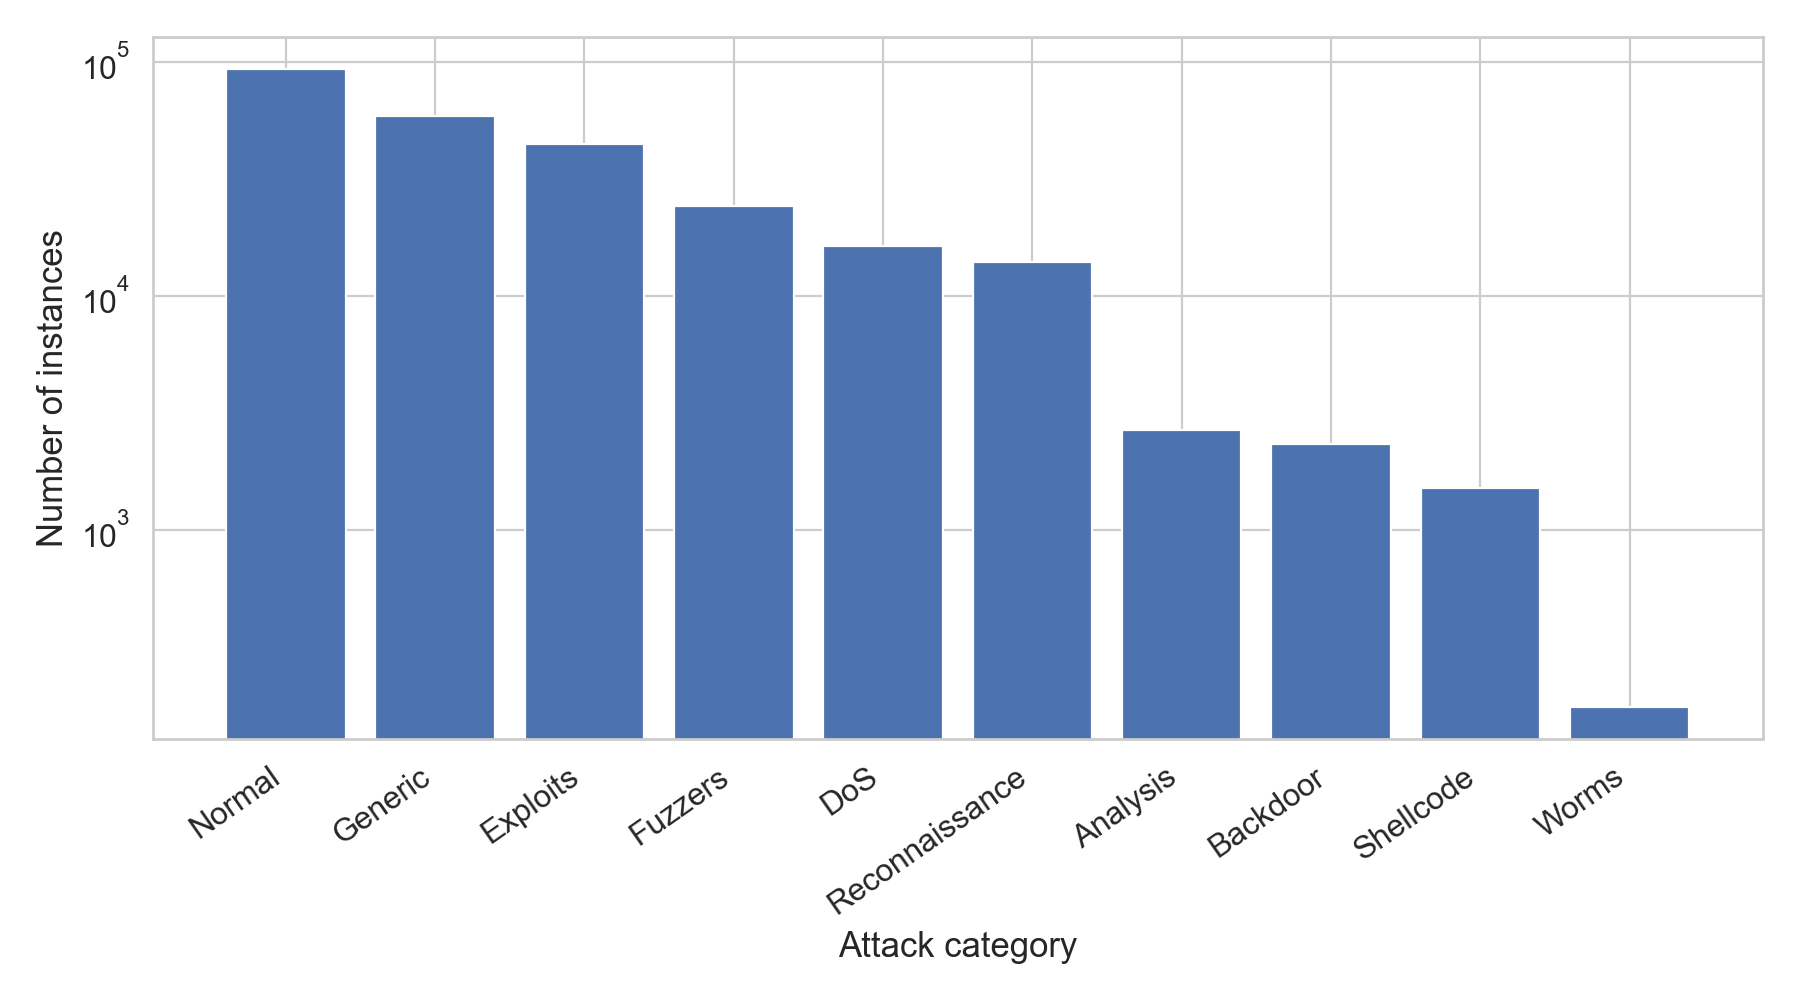
\includegraphics[width=\columnwidth]{figures/report/01_class_distribution.png}
\caption{Distribution of instances across attack categories, shown on a logarithmic scale.}
\label{fig:class-distribution}
\end{figure}

Exploratory analysis identified three additional properties relevant to the preprocessing pipeline described in Section~\ref{sec:implementation}. First, the service feature contains a placeholder value, denoted \texttt{?}, for 54.85 percent of instances. The rate of occurrence of this placeholder value varies across attack categories, ranging from 1.55 percent for the Generic category to 100 percent for the Shellcode category, as shown in Table~\ref{tab:service-missing}. Second, duplicate flow records, defined as rows identical to at least one other row across all features excluding the row identifier, account for 44.18 percent of all instances. The rate of duplication varies across attack categories, ranging from 3.45 percent for the Worms category to 96.48 percent for the Generic category, as shown in Figure~\ref{fig:duplicates}. Third, the protocol feature contains 133 distinct categories, of which 123 categories each account for fewer than 0.1 percent of all instances.

\begin{table}[t]
\caption{Rate of the missing service placeholder value by attack category}
\label{tab:service-missing}
\centering
\begin{tabular}{lr}
\toprule
Attack category & Missing service (\%) \\
\midrule
Shellcode & 100.00 \\
Backdoor & 95.28 \\
Fuzzers & 90.65 \\
Denial of Service & 84.66 \\
Reconnaissance & 84.22 \\
Analysis & 78.93 \\
Normal & 68.70 \\
Exploits & 51.76 \\
Worms & 14.94 \\
Generic & 1.55 \\
\bottomrule
\end{tabular}
\end{table}

\begin{figure}[t]
\centering
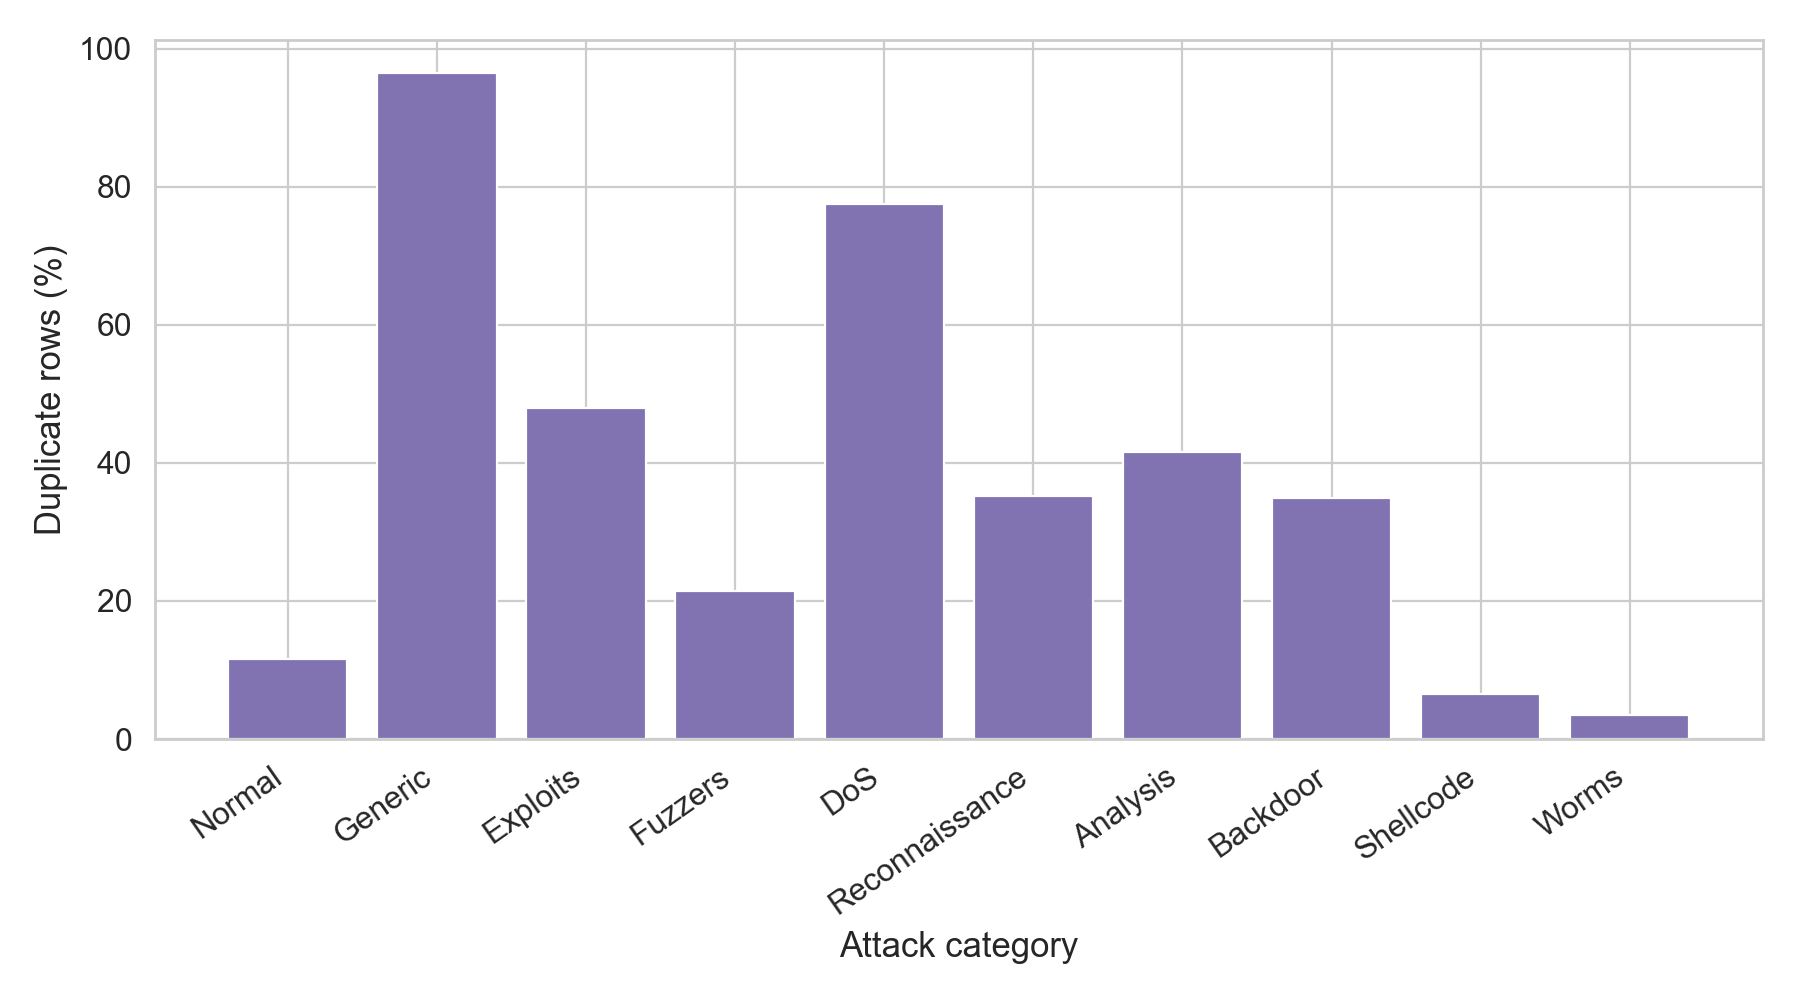
\includegraphics[width=\columnwidth]{figures/report/02_duplicate_rate_by_class.png}
\caption{Rate of flow records that have at least one duplicate, by attack category.}
\label{fig:duplicates}
\end{figure}

\subsection{Evaluation Metrics}
Classifier performance is reported using precision, recall, and the F1-score. For a given class, precision is the proportion of instances predicted as that class that are correctly classified, and recall is the proportion of instances truly belonging to that class that are correctly classified. The F1-score is the harmonic mean of precision and recall for a given class, given by
\begin{equation}
F1 = \frac{2 \cdot \text{precision} \cdot \text{recall}}{\text{precision} + \text{recall}}.
\end{equation}
The macro F1-score is the unweighted mean of the per-class F1-score across all classes, and the weighted F1-score is the mean of the per-class F1-score weighted by the number of instances in each class. Macro F1-score is applied as the primary tuning and comparison metric in this report, because accuracy and weighted F1-score are dominated by the majority categories under the class imbalance described above.

Stratified $k$-fold CV partitions the training data into $k$ folds, such that each fold preserves the overall class distribution. A model is trained on $k-1$ folds and evaluated on the remaining fold, repeated $k$ times so that every fold serves as the validation fold exactly once.

\section{Implementation}
\label{sec:implementation}
This section describes the preprocessing pipeline and the configuration of the two ensemble classifiers prior to tuning. Each preprocessing decision is justified by a finding reported in Section~\ref{sec:background}.

\subsection{Preprocessing Pipeline}
The row identifier feature was removed prior to training, because this feature carried no predictive information. The \texttt{is\_ftp\_login} feature, documented as a binary indicator, was observed to contain the values 0, 1, 2, and 4. This feature was binarised by mapping any value greater than 0 to 1, consistent with the documented semantics of the feature.

The placeholder value present in the service feature was retained as an explicit category rather than treated as missing data subject to imputation, because the rate of occurrence of the placeholder value varied across attack categories, as shown in Table~\ref{tab:service-missing}. This variation indicated that the placeholder value carried information relevant to the prediction task.

The protocol feature was transformed prior to encoding by grouping categories that each accounted for fewer than 0.1 percent of instances into a single category. This grouping reduced the number of distinct protocol categories from 133 to 11, including the newly introduced grouped category.

The three nominal features, protocol, service, and connection state, were encoded using one-hot encoding. One-hot encoding was selected over ordinal encoding because none of the three features possessed a natural ordering. An ordinal encoding would have introduced a false ordering that a tree-based split could exploit spuriously.

No feature scaling was applied prior to training the RF and GBM classifiers. Tree-based classifiers partition the feature space using threshold comparisons on individual features, and the position of a threshold is unaffected by a monotonic transformation applied to a feature, such as scaling.

Duplicate flow records identified in Section~\ref{sec:background} were not removed prior to training. The rate of duplication varied across attack categories, and removal of duplicate records would have disproportionately reduced the number of training instances available for attack categories with a high duplication rate, without a clear justification that the duplicate records resulted from a data collection error rather than genuinely repeated attack traffic patterns.

The dataset was partitioned into a training partition containing 80 percent of instances and a test partition containing the remaining 20 percent of instances, using stratified sampling with respect to the target attribute. Table~\ref{tab:split-balance} confirms that the stratified partitioning produced near-identical class proportions in both partitions.

\begin{table}[t]
\caption{Class proportions in the training and test partitions}
\label{tab:split-balance}
\centering
\begin{tabular}{lrr}
\toprule
Attack category & Training (\%) & Test (\%) \\
\midrule
Normal & 36.09 & 36.09 \\
Generic & 22.85 & 22.85 \\
Exploits & 17.28 & 17.28 \\
Fuzzers & 9.41 & 9.41 \\
Denial of Service & 6.35 & 6.35 \\
Reconnaissance & 5.43 & 5.43 \\
Analysis & 1.04 & 1.04 \\
Backdoor & 0.90 & 0.90 \\
Shellcode & 0.59 & 0.59 \\
Worms & 0.07 & 0.07 \\
\bottomrule
\end{tabular}
\end{table}

Note that duplicate flow records were present before the 80/20 split was applied, and duplicate copies were therefore distributed across both the training partition and the test partition. This property is relevant to the discussion of CV reliability in Section~\ref{sec:empirical}.

\subsection{Decision Tree and $k$ Nearest Neighbours Classifiers}
The DT classifier and the kNN classifier were constructed in a previous assignment on the same dataset, prior to the 80/20 held-out split described above. Both classifiers were tuned through a grid search combined with 5-fold stratified CV, evaluated using CV predictions obtained across the full dataset of 257,673 instances. This evaluation protocol differs from the held-out test partition protocol applied to the RF and GBM classifiers in the present report, and this difference is addressed explicitly in Section~\ref{sec:results}.

The tuned DT classifier applied the entropy splitting criterion, a maximum depth of 20, a minimum of 2 samples required to split an internal node, a minimum of 5 samples required at a leaf node, and balanced class weighting. The tuned kNN classifier applied 5 neighbours, the Euclidean distance metric, and distance-weighted voting.

\subsection{Random Forest Classifier}
The RF classifier was configured with the number of trees, the maximum tree depth, the minimum number of samples required to split an internal node, the minimum number of samples required at a leaf node, the number of features considered at each split, and the class weighting scheme as tunable hyperparameters. The tuning of these hyperparameters is described in Section~\ref{sec:empirical}.

\subsection{Gradient Boosting Classifier}
The histogram-based GBM classifier was applied in place of the standard gradient boosting implementation. The standard implementation constructs trees strictly sequentially, with no parallelisation available within a single model fit. Sequential construction made the standard implementation computationally prohibitive on the 206,138 training instances available. The histogram-based implementation discretises continuous features into bins prior to training, reducing the computational cost of split evaluation while retaining the sequential property central to boosting.

Class imbalance was addressed for the GBM classifier by supplying an inverse-frequency sample weight to each training instance, computed as
\begin{equation}
w_i = \frac{N}{K \cdot N_{y_i}},
\end{equation}
where $N$ is the total number of training instances, $K$ is the number of classes, and $N_{y_i}$ is the number of training instances belonging to the class of instance $i$. Under this weighting scheme, the Worms category received a weight of approximately 148.3, and the Normal category received a weight of approximately 0.277. Sample weighting was applied in preference to the native class weighting parameter available in the applied library, to match the exact inverse-frequency formula stated above.

The histogram-based GBM classifier applied in this report does not expose an impurity-based feature importance measure, in contrast to the RF classifier. Permutation importance was computed instead for the GBM classifier, by measuring the reduction in macro F1-score observed when the values of a single feature were randomly permuted across a subsample of 20,000 training instances, repeated 5 times per feature. This subsample was drawn from the training partition rather than the test partition, which is noted as a limitation, because permutation importance computed on training data can overstate the importance of features that the model has overfitted to.

\section{Empirical Process}
\label{sec:empirical}
This section describes the empirical process followed to tune the RF and GBM classifiers and to answer four research questions established prior to tuning. The four research questions addressed the effect of the number of trees on the RF classifier, the effect of maximum tree depth on the RF classifier, the effect of learning rate on the GBM classifier, and the effect of class weighting on the RF classifier. Each research question was investigated using 5-fold stratified CV on the training partition, with macro F1-score as the evaluation metric.

\subsection{Effect of the Number of Trees}
The first research question investigated whether an increase in the number of trees in the RF classifier reduced the variance of the ensemble prediction without a corresponding increase in overfitting. The number of trees was varied across the values 10, 25, 50, 100, 200, and 300, with balanced class weighting applied. Figure~\ref{fig:val-rf-nestimators} shows the training and validation macro F1-score obtained for each value. The validation score increased from 0.548 at 10 trees to 0.566 at 300 trees. The majority of the improvement occurred between 10 and 100 trees. The fold-to-fold standard deviation of the validation score decreased from 0.011 at 10 trees to 0.008 at 300 trees, indicating a modest reduction in variance across folds as the number of trees increased. The gap between the training score and the validation score remained approximately 0.19 across all values tested, indicating that the increase in the number of trees reduced neither the bias of the ensemble nor the training-validation gap, consistent with the theoretical expectation that increasing the number of trees in a bagged ensemble primarily affects variance rather than bias.

\begin{figure}[t]
\centering
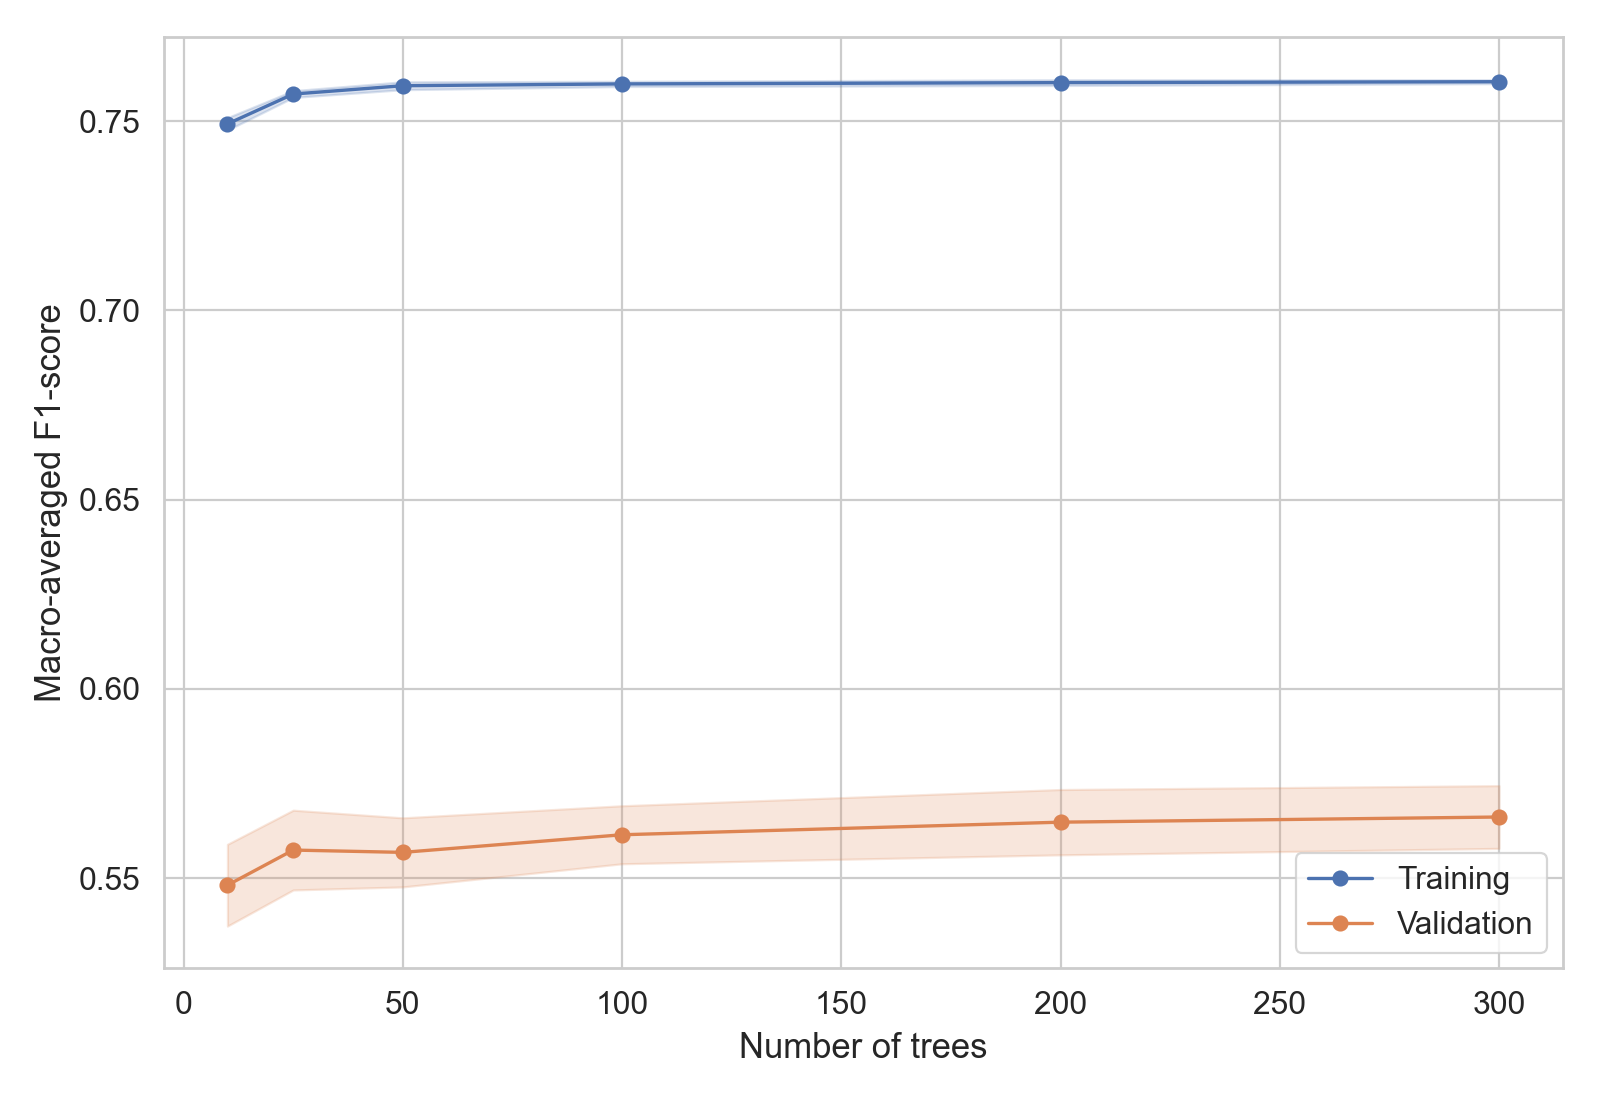
\includegraphics[width=\columnwidth]{figures/report/03a_validation_curve_rf_n_estimators.png}
\caption{Training and validation macro F1-score of the RF classifier as a function of the number of trees.}
\label{fig:val-rf-nestimators}
\end{figure}

\subsection{Effect of Maximum Tree Depth}
The second research question investigated whether maximum tree depth controlled the trade-off between bias and variance in the RF classifier. The maximum tree depth was varied across the values 2, 4, 6, 8, 12, 16, 20, and an unconstrained depth, with the number of trees held at 100. Figure~\ref{fig:val-rf-maxdepth} shows the results. The training score increased monotonically from 0.254 at a maximum depth of 2 to 0.760 at an unconstrained depth. The validation score increased from 0.254 to a peak of 0.572 at a maximum depth of 20, and then decreased slightly to 0.561 at an unconstrained depth. The gap between the training score and the validation score increased from near zero at a maximum depth of 2 to 0.198 at an unconstrained depth, demonstrating the expected trade-off between bias and variance as tree depth increased.

\begin{figure}[t]
\centering
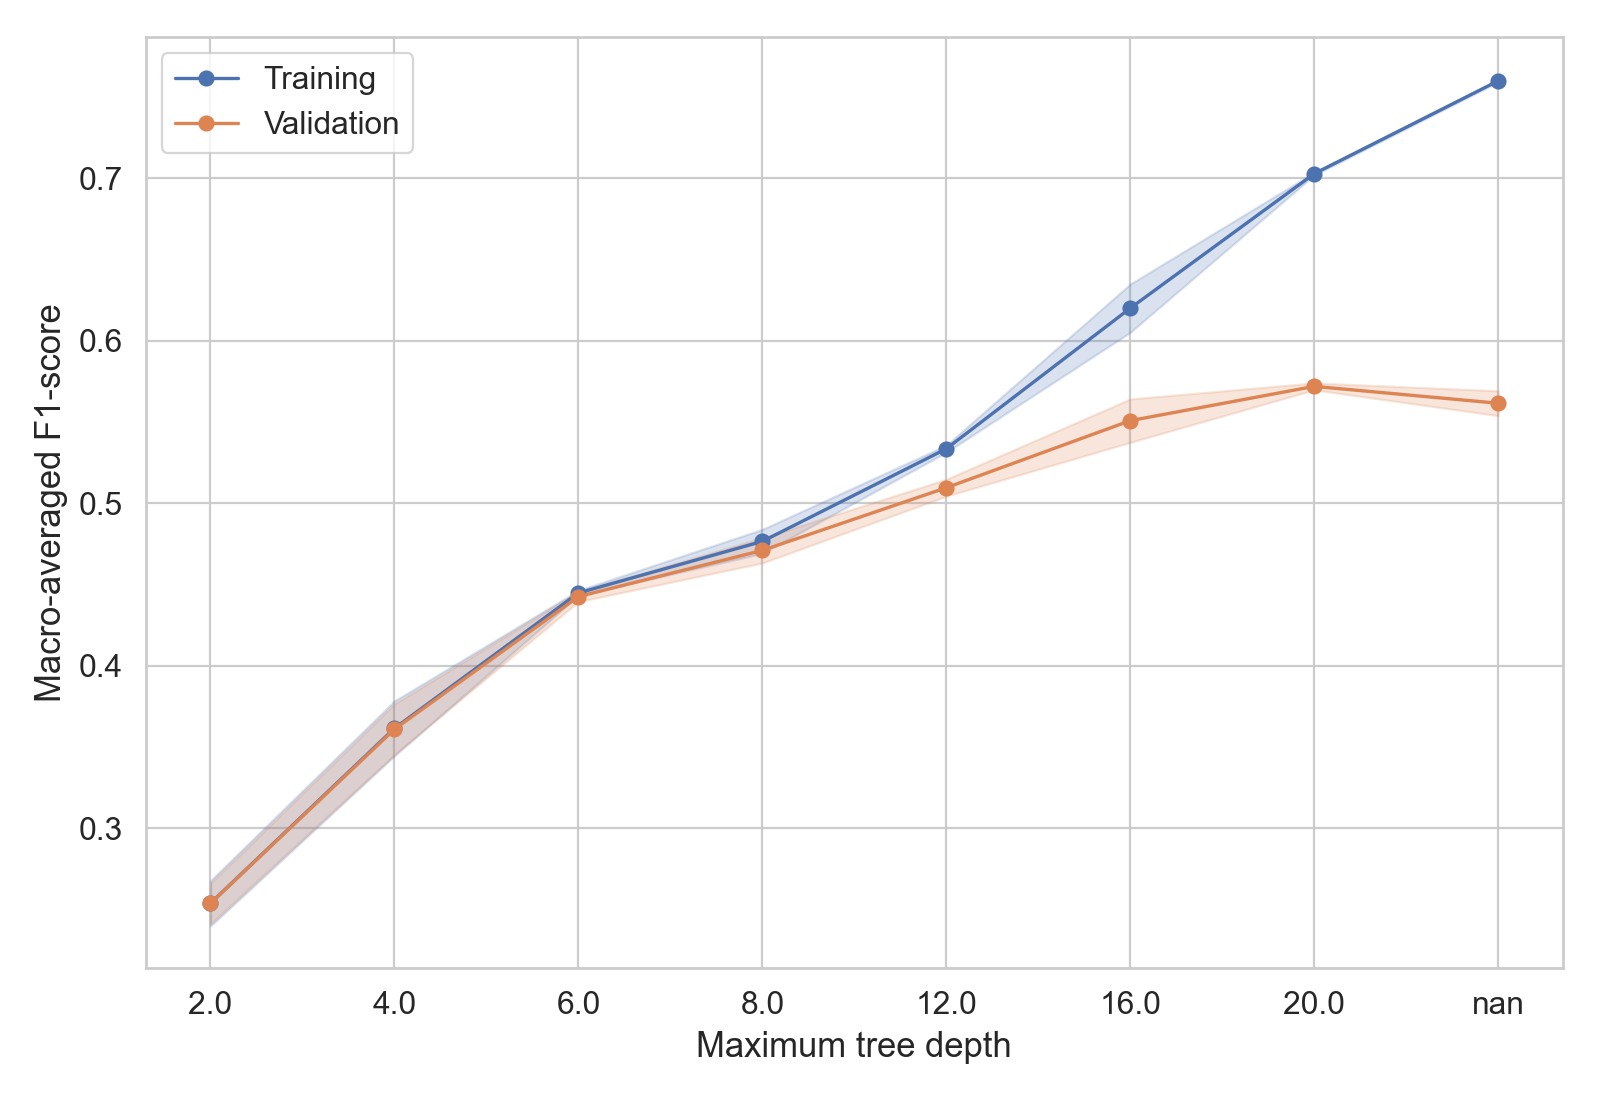
\includegraphics[width=\columnwidth]{figures/report/03b_validation_curve_rf_max_depth.png}
\caption{Training and validation macro F1-score of the RF classifier as a function of maximum tree depth. The rightmost point corresponds to an unconstrained maximum depth.}
\label{fig:val-rf-maxdepth}
\end{figure}

\subsection{Effect of Learning Rate}
The third research question investigated whether the learning rate of the GBM classifier behaved as predicted by boosting theory. The learning rate was varied across the values 0.01, 0.05, 0.1, 0.2, and 0.3, with the maximum number of boosting iterations fixed at 100 and early stopping disabled. Figure~\ref{fig:val-gbm-lr} shows the results. The validation score decreased monotonically from 0.541 at a learning rate of 0.01 to 0.418 at a learning rate of 0.3. The training score also decreased over the same range, from 0.582 to 0.430. This simultaneous decrease in both the training score and the validation score at high learning rates indicates optimisation instability at high learning rates rather than overfitting at low learning rates, because overfitting would be expected to produce a high training score together with a lower validation score. The large sample weights applied to minority categories, described in Section~\ref{sec:implementation}, are a plausible contributor to this instability, because a large weight applied to a small number of instances can cause a large single-step update to the ensemble prediction at a high learning rate.

\begin{figure}[t]
\centering
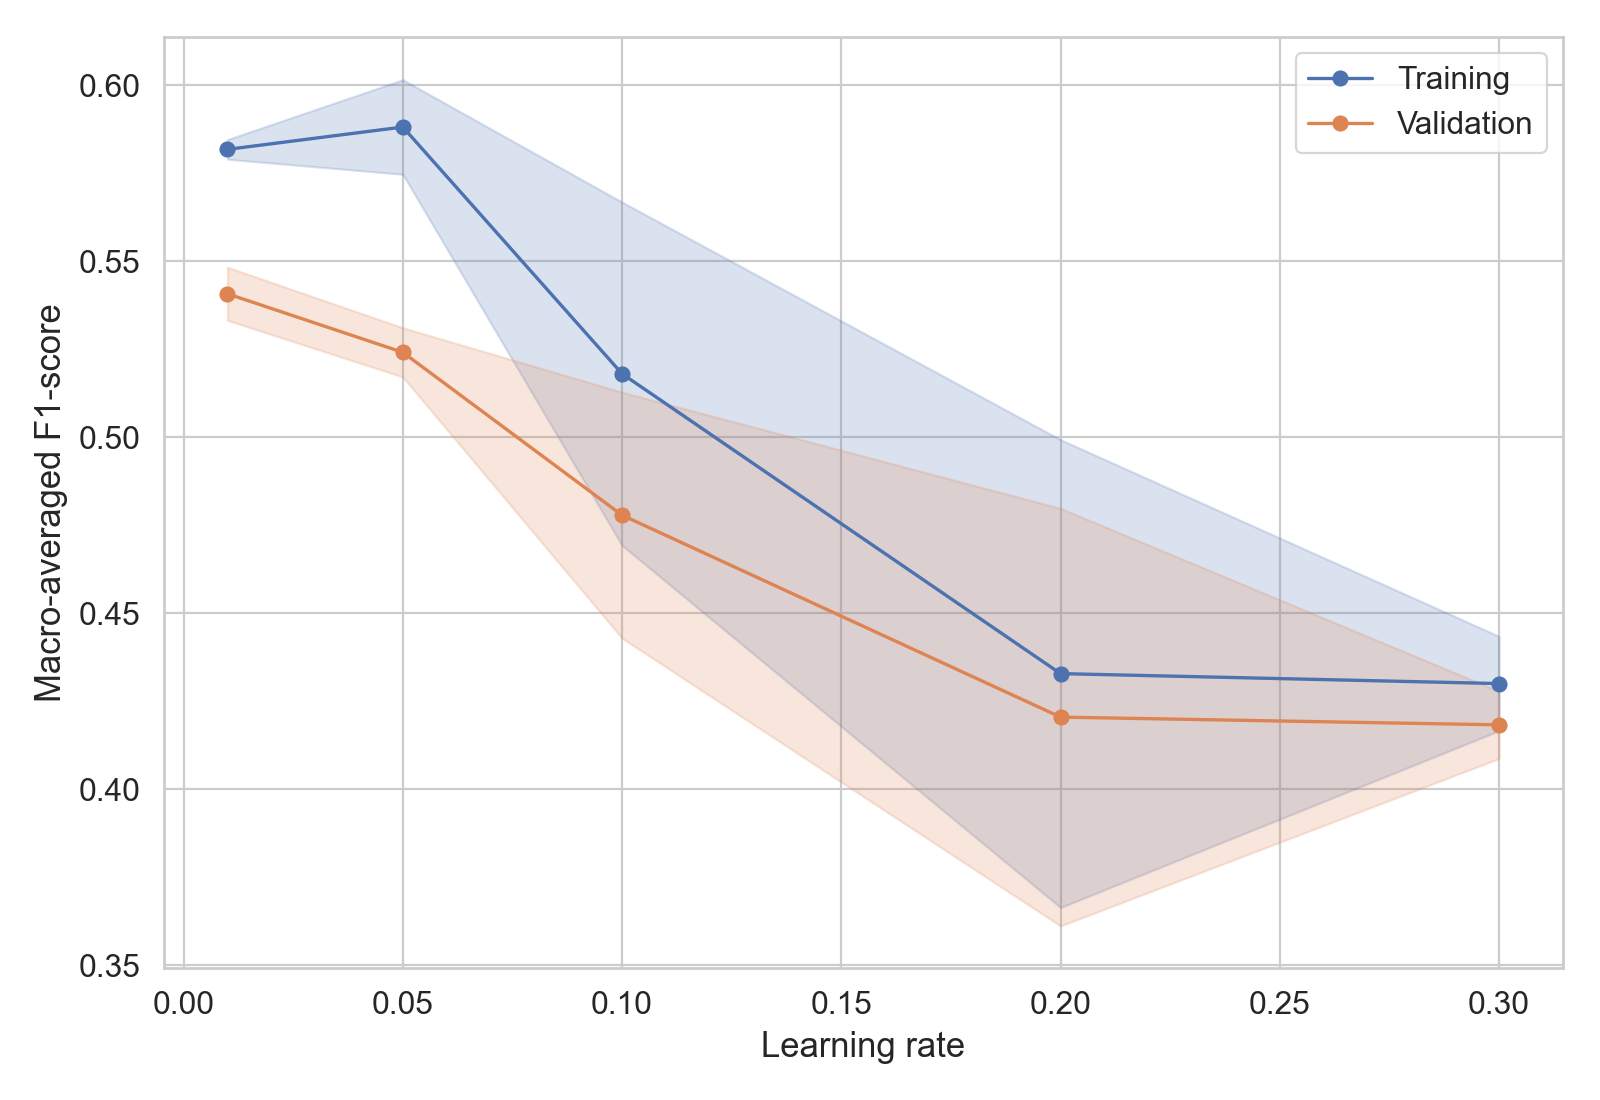
\includegraphics[width=\columnwidth]{figures/report/04a_validation_curve_gbm_learning_rate.png}
\caption{Training and validation macro F1-score of the GBM classifier as a function of learning rate, with the maximum number of boosting iterations fixed at 100.}
\label{fig:val-gbm-lr}
\end{figure}

\subsection{Effect of Class Weighting}
The fourth research question investigated whether balanced class weighting improved the detection of minority attack categories relative to unweighted training, using the RF classifier with 100 trees. Table~\ref{tab:classweight} shows the mean and standard deviation of the macro F1-score across 5 CV folds for both configurations. The unweighted configuration achieved a marginally higher mean macro F1-score of 0.567, compared with 0.561 for the balanced configuration. Balanced class weighting therefore did not improve overall macro F1-score on this dataset when applied to the RF classifier. The final tuned RF classifier nonetheless applied balanced subsample class weighting, because the hyperparameter search described in Section~\ref{subsec:final-search} selected this configuration on the basis of overall cross-validated macro F1-score, and the two results are not directly comparable because the final search varied several hyperparameters jointly rather than class weighting alone.

\begin{table}[t]
\caption{Macro F1-score for unweighted and balanced class weighting, 5-fold CV}
\label{tab:classweight}
\centering
\begin{tabular}{lrr}
\toprule
& Unweighted & Balanced \\
\midrule
Mean & 0.567 & 0.561 \\
Standard deviation & 0.006 & 0.008 \\
\bottomrule
\end{tabular}
\end{table}

\subsection{Final Hyperparameter Search}
\label{subsec:final-search}
Following the four validation curves described above, a randomised search over 25 candidate configurations was conducted independently for each ensemble classifier, using 5-fold stratified CV and macro F1-score as the scoring metric.

The RF search identified a best configuration of 400 trees, a maximum depth of 16, a minimum split sample count of 2, a minimum leaf sample count of 2, an unrestricted number of features considered at each split, and balanced subsample class weighting, achieving a CV macro F1-score of 0.586. An unrestricted number of features considered at each split removes the per-split feature subsampling that distinguishes a random forest from plain bagging of decision trees, as described in Section~\ref{sec:background}. The tuned RF classifier applied in this report is therefore better described as a bagged ensemble of deep decision trees, rather than a random forest in the strict sense, and this is discussed further in Section~\ref{sec:results}.

The GBM search identified a best configuration of 150 boosting iterations, a learning rate of 0.05, a maximum tree depth of 6, a maximum of 15 leaf nodes, a minimum leaf sample count of 20, and no L2 regularisation, achieving a CV macro F1-score of 0.702.

The CV macro F1-score obtained for the best GBM configuration is substantially higher than the macro F1-score subsequently obtained on the held-out test partition, as reported in Section~\ref{sec:results}. This discrepancy is discussed in Section~\ref{subsec:cv-gap}.

\section{Results and Discussion}
\label{sec:results}
This section presents the results obtained on the held-out test partition for the RF and GBM classifiers, followed by a comparison against the DT and kNN classifiers constructed in a previous assignment. The section then discusses per-category performance, the CV-test discrepancy, feature importance, and computational cost.

\subsection{Overall Test Set Performance}
Table~\ref{tab:overall-comparison} shows the overall performance of all four classifiers. The RF classifier achieves the highest macro F1-score among the four classifiers, at 0.598. The DT classifier achieves a macro F1-score of 0.588, within 0.010 of the RF classifier. The GBM classifier achieves a macro F1-score of 0.565, and the kNN classifier achieves the lowest macro F1-score among the four classifiers, at 0.508. The DT and kNN results in Table~\ref{tab:overall-comparison} were obtained under a CV protocol on the full dataset rather than the held-out test protocol applied to the RF and GBM classifiers, as described in Section~\ref{sec:implementation}, and the comparison should be interpreted with this difference in mind.

\begin{table}[t]
\caption{Overall performance of all four classifiers. DT and kNN results are 5-fold CV estimates on the full dataset; RF and GBM results are held-out test estimates.}
\label{tab:overall-comparison}
\centering
\begin{tabular}{lrrr}
\toprule
Classifier & Macro F1 & Weighted F1 & Accuracy \\
\midrule
RF & 0.598 & 0.790 & 0.765 \\
GBM & 0.565 & 0.779 & 0.753 \\
DT & 0.588 & 0.795 & 0.767 \\
kNN & 0.508 & 0.783 & 0.786 \\
\bottomrule
\end{tabular}
\end{table}

\begin{figure}[t]
\centering
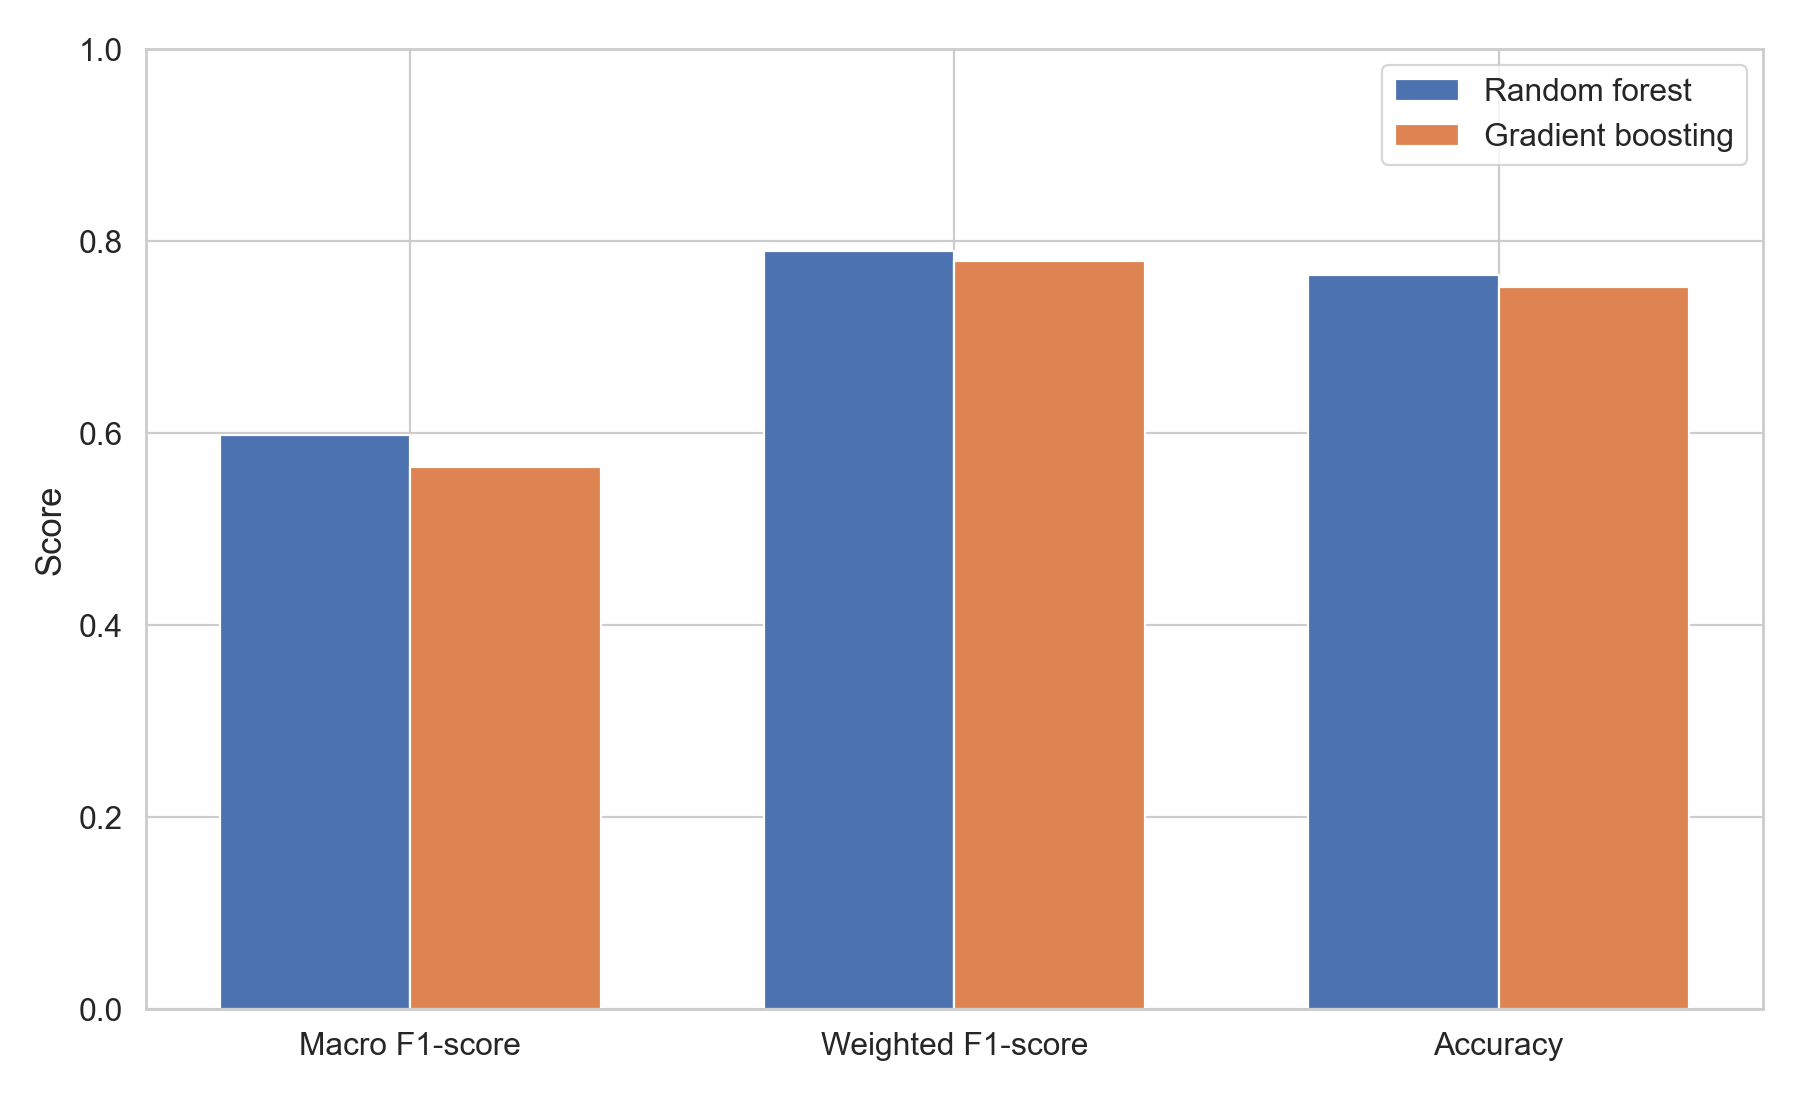
\includegraphics[width=\columnwidth]{figures/report/10_overall_model_comparison.png}
\caption{Test set macro F1-score, weighted F1-score, and accuracy for the RF and GBM classifiers.}
\label{fig:overall-comparison}
\end{figure}

The ranking of the four classifiers by macro F1-score does not match the ranking by accuracy. The kNN classifier achieves the highest accuracy among the four classifiers, at 0.786, despite achieving the lowest macro F1-score. The severe class imbalance described in Section~\ref{sec:background} allows a classifier biased toward the majority categories to achieve high accuracy while performing poorly on the minority attack categories, and this result demonstrates that outcome directly.

The small margin separating the RF classifier from the DT classifier indicates that a single, well-tuned decision tree achieves a level of performance on this dataset close to that of a bagged ensemble of 400 such trees. The RF classifier nonetheless achieves a higher macro F1-score than the single DT classifier, consistent with the theoretical expectation that variance reduction through bagging improves generalisation performance relative to a single base learner. The kNN classifier achieves the lowest macro F1-score among the four classifiers. This result is consistent with the high dimensionality of the one-hot encoded feature space described in Section~\ref{sec:implementation}, in which a large number of sparse binary features can dilute the contribution of informative continuous features to a Euclidean distance calculation~\cite{beyer1999nearest}.

\subsection{Per-Category Performance}
Figure~\ref{fig:per-class-f1} shows the F1-score achieved by the RF and GBM classifiers for each of the 10 attack categories. The Generic category achieves the highest F1-score for both classifiers, at 0.988 for the RF classifier and 0.987 for the GBM classifier. The Backdoor and Analysis categories achieve the lowest F1-scores for both classifiers. The RF classifier achieves an F1-score of 0.094 for the Backdoor category and 0.139 for the Analysis category. The GBM classifier achieves an F1-score of 0.144 for the Backdoor category and 0.182 for the Analysis category.

\begin{figure}[t]
\centering
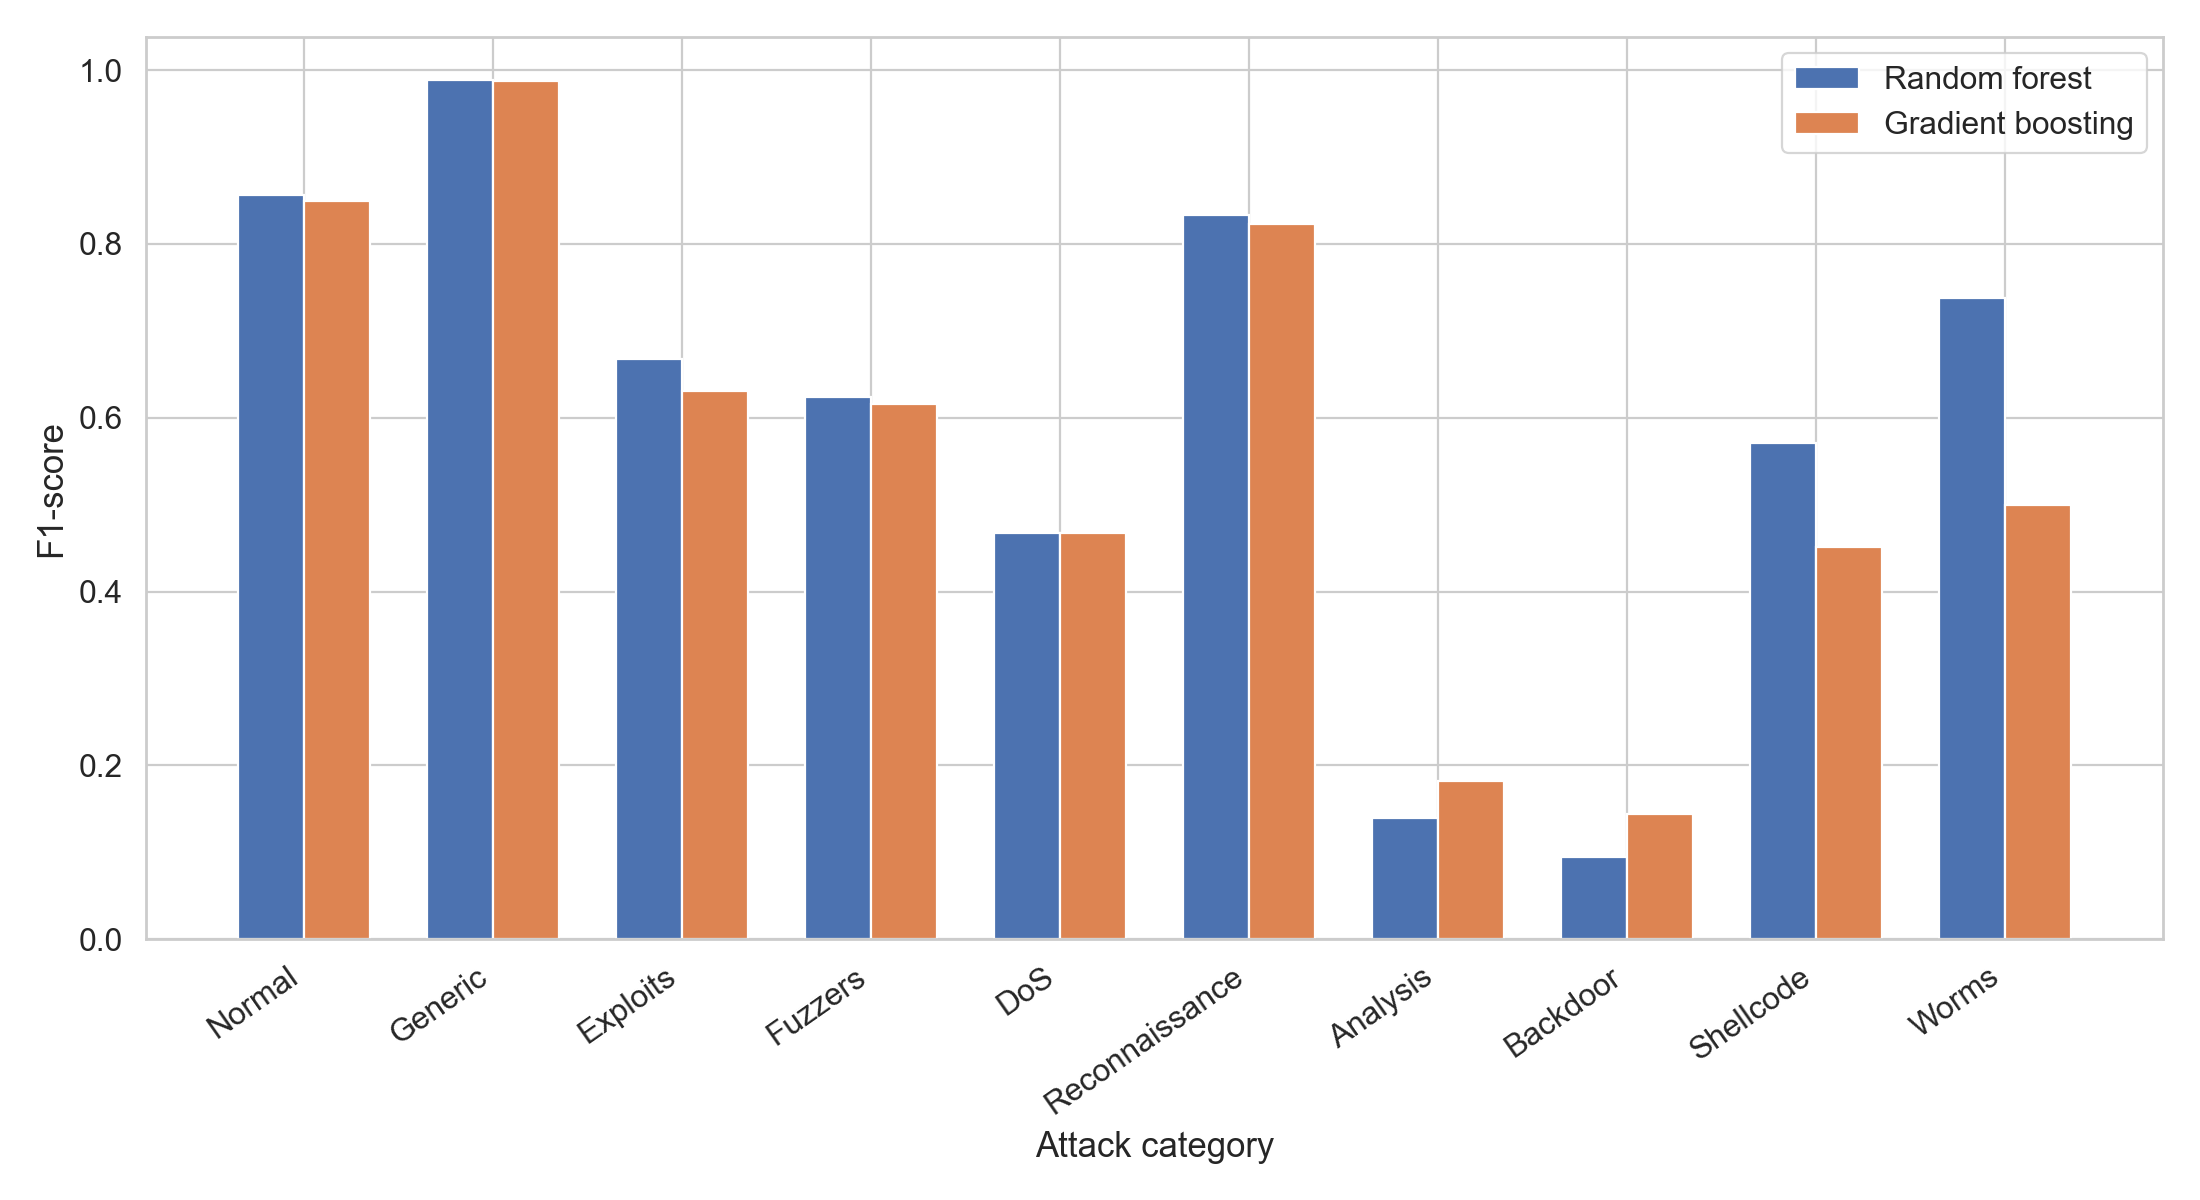
\includegraphics[width=\columnwidth]{figures/report/07_per_class_f1_comparison.png}
\caption{F1-score by attack category for the RF and GBM classifiers.}
\label{fig:per-class-f1}
\end{figure}

Table~\ref{tab:confusion-rf} shows the rows of the RF confusion matrix corresponding to the Backdoor and Analysis categories, restricted to the columns receiving the largest number of misclassified instances. Of 466 Backdoor test instances, 151 instances were classified as DoS and 41 instances were classified as Exploits. Of 535 Analysis test instances, 161 instances were classified as DoS and 47 instances were classified as Exploits. The Exploits and DoS categories therefore account for a substantial share of the misclassifications of both the Backdoor and Analysis categories, supporting the explanation that these three categories share overlapping feature distributions.

\begin{table}[t]
\caption{Selected RF confusion matrix entries for the Backdoor and Analysis categories (test partition)}
\label{tab:confusion-rf}
\centering
\begin{tabular}{lrrr}
\toprule
True category & Predicted DoS & Predicted Exploits & Support \\
\midrule
Backdoor & 151 & 41 & 466 \\
Analysis & 161 & 47 & 535 \\
\bottomrule
\end{tabular}
\end{table}

Figure~\ref{fig:backdoor-analysis-pr} shows the precision and recall achieved by the RF and GBM classifiers for the Backdoor and Analysis categories. The RF classifier achieves a precision of 0.063 and a recall of 0.189 for the Backdoor category, while the GBM classifier achieves a precision of 0.088 and a recall of 0.399 for the same category. The GBM classifier achieves more than double the recall of the RF classifier on the Backdoor category. The inverse-frequency sample weighting applied during the training of the GBM classifier assigned the Backdoor category a weight of approximately 11.1. This weighting shifted the decision boundary of the GBM classifier toward higher recall at the cost of precision for this category.

\begin{figure}[t]
\centering
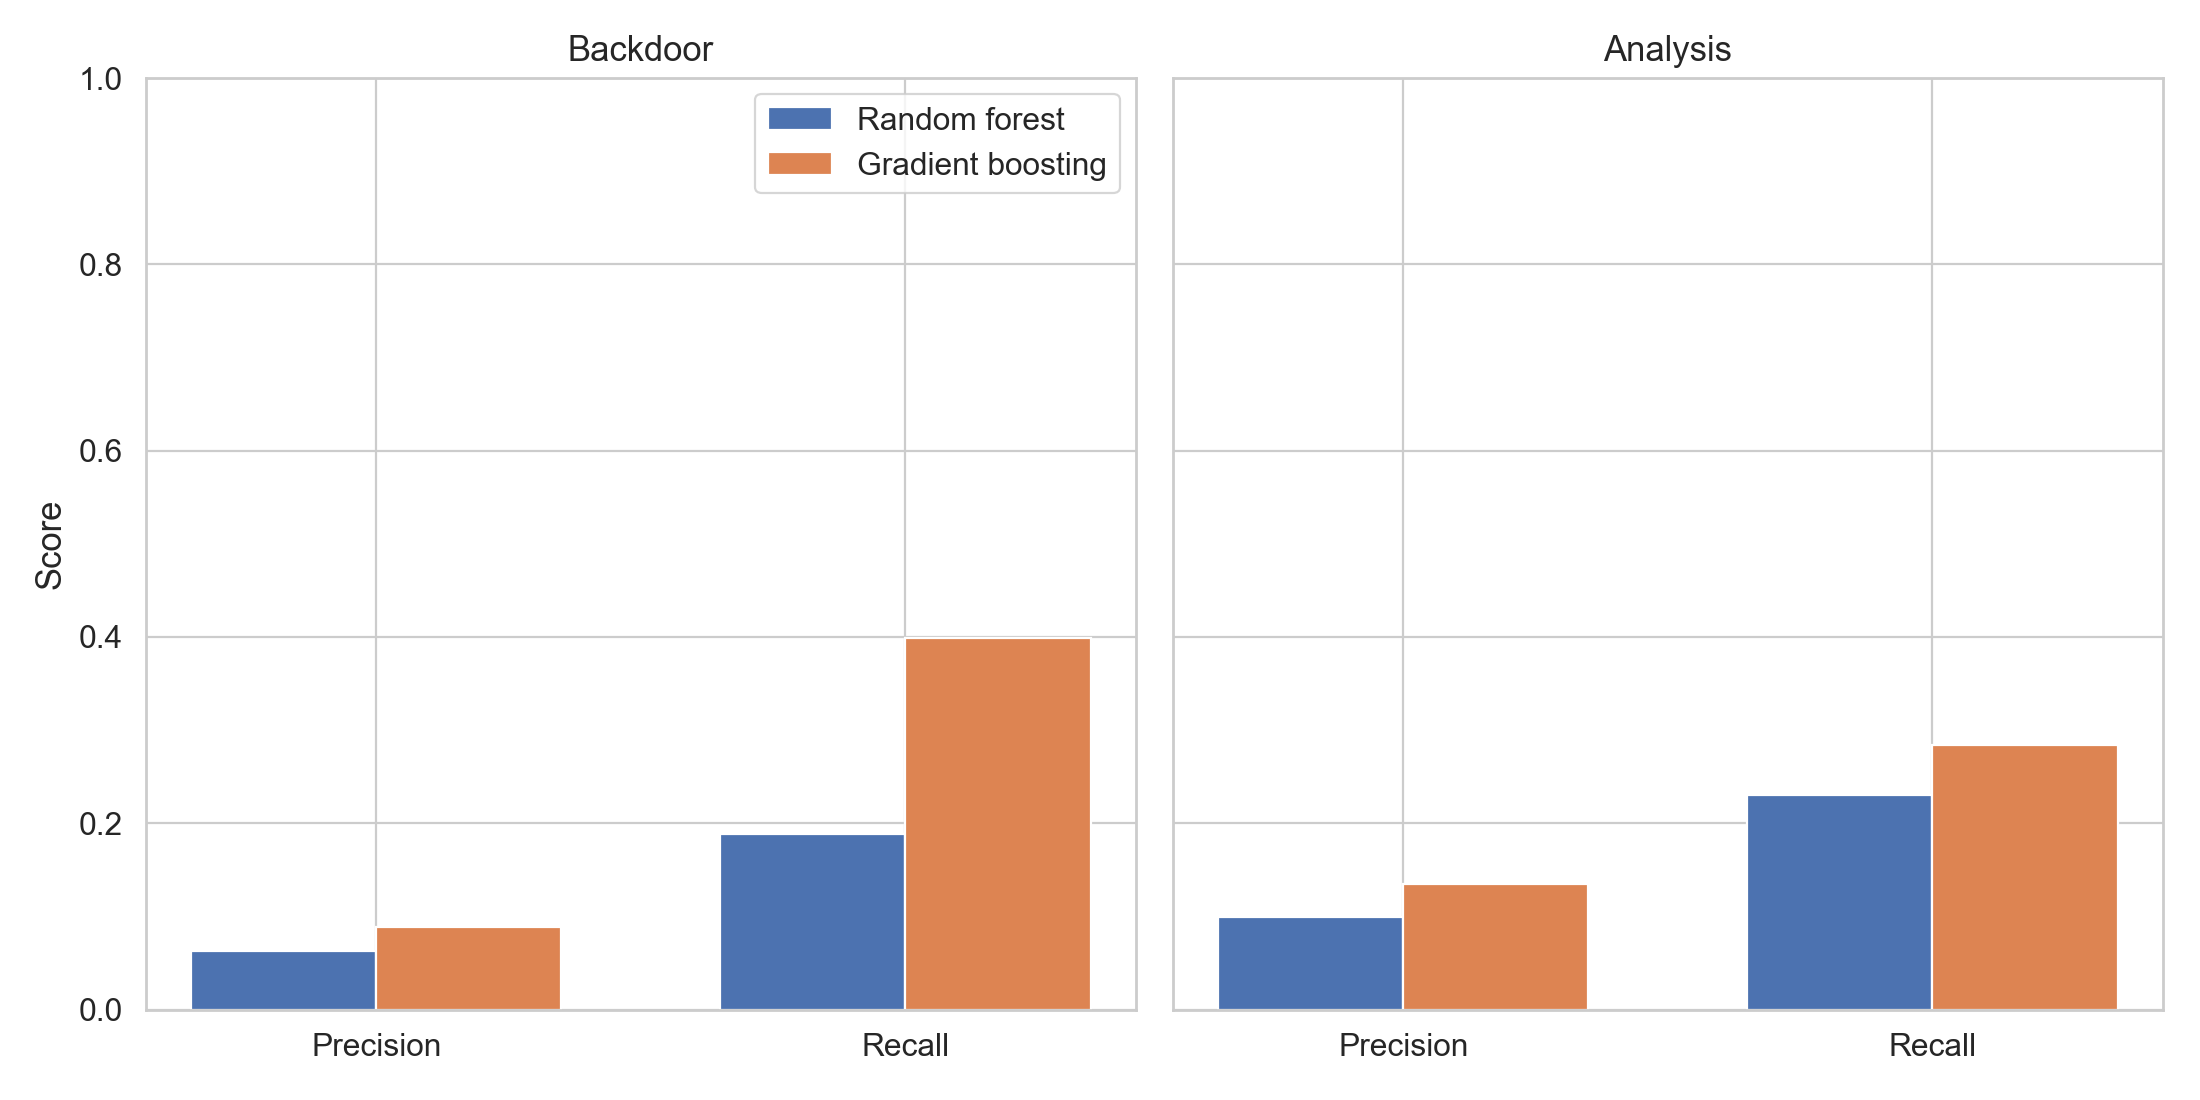
\includegraphics[width=\columnwidth]{figures/report/08_backdoor_analysis_precision_recall.png}
\caption{Precision and recall for the Backdoor and Analysis categories.}
\label{fig:backdoor-analysis-pr}
\end{figure}

The Backdoor category contains 2,329 training instances and the Analysis category contains 2,677 training instances. The combination of a low number of training instances with the confusion against the Exploits and DoS categories shown in Table~\ref{tab:confusion-rf} is identified as the primary limitation affecting the performance of both ensemble classifiers on these two categories. This limitation was not resolved through class weighting, because the ablation study reported in Table~\ref{tab:classweight} found no improvement in overall macro F1-score when balanced weighting was applied to the RF classifier.

Examination of the DT and kNN results confirmed that this weakness is not specific to the two ensemble classifiers. The DT classifier achieves an F1-score of 0.085 for the Backdoor category and 0.109 for the Analysis category, and the kNN classifier achieves an F1-score of 0.066 for the Backdoor category and 0.184 for the Analysis category. The consistent weakness observed across four classifiers constructed using four distinct learning algorithms supports the conclusion that the low performance on the Backdoor and Analysis categories results from a property of the dataset, rather than from a limitation specific to any single classifier.

\subsection{Discrepancy Between Cross-Validation and Test Performance}
\label{subsec:cv-gap}
Figure~\ref{fig:cv-vs-test} shows the best CV macro F1-score obtained during the randomised hyperparameter search alongside the corresponding macro F1-score obtained on the held-out test partition, for the RF and GBM classifiers. The RF classifier achieves a CV score of 0.586 and a test score of 0.598, a consistent estimate of generalisation performance. The GBM classifier achieves a CV score of 0.702 and a test score of 0.565, a substantial overestimate of generalisation performance during CV.

\begin{figure}[t]
\centering
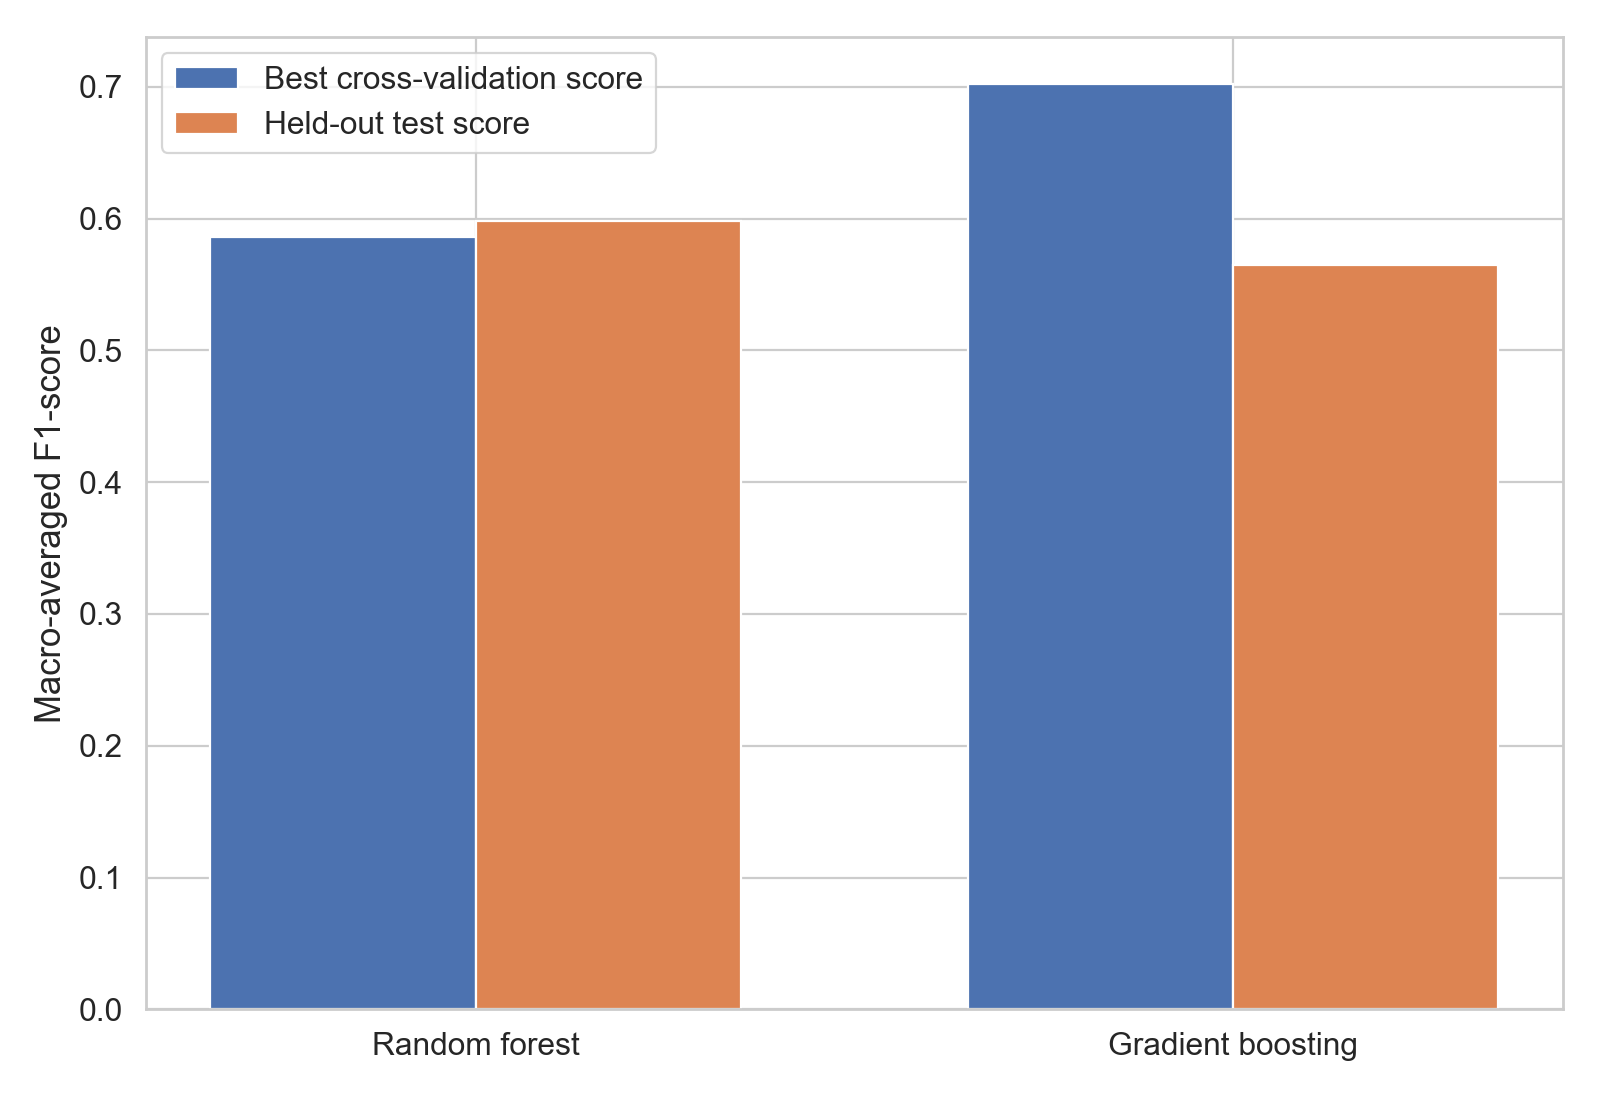
\includegraphics[width=\columnwidth]{figures/report/06_cv_vs_test_gap.png}
\caption{Best CV macro F1-score compared with test set macro F1-score.}
\label{fig:cv-vs-test}
\end{figure}

This gap was initially attributed to duplicate flow records being distributed across training and validation folds during stratified CV. This explanation does not fully account for the observed gap, because duplicate flow records were present before the 80/20 split was applied, as noted in Section~\ref{sec:implementation}, and duplicate copies were therefore distributed across the training partition and the test partition in the same manner as across CV folds. Fold-level leakage from duplication would therefore be expected to inflate both the CV estimate and the test estimate by a similar amount, which is not what was observed. The RF classifier, cross-validated on the same folds and the same duplicated training data, shows no comparable gap. A software or evaluation error affecting the GBM search, such as the scorer applied during the randomised search differing from the scorer applied during final test evaluation, is considered a more likely explanation than duplication-driven leakage alone, but this explanation has not been confirmed by inspection of the implementation. The gap between the CV estimate and the test estimate for the GBM classifier is therefore reported as an unresolved limitation of the empirical process, and the test set macro F1-score of 0.565 is taken as the reliable estimate of GBM generalisation performance for the purpose of the comparison in this report.

\subsection{Feature Importance}
Figure~\ref{fig:feature-importance} shows the most important features identified for each classifier, normalised to sum to 1 within each classifier to allow a visual comparison between the impurity-based importance measure applied to the RF classifier and the permutation-based importance measure applied to the GBM classifier. Both classifiers identify the source bytes feature, the source time-to-live feature, the source mean packet size feature, and the domain name system service indicator feature among the most important features. This agreement between two independently tuned classifiers, computed using different importance measures, corroborates the relevance of these four features to the prediction task. Impurity-based importance is known to be biased toward high-cardinality and continuous features~\cite{strobl2007bias}, and this bias should be considered when interpreting the RF importance values in Figure~\ref{fig:feature-importance}.

\begin{figure}[t]
\centering
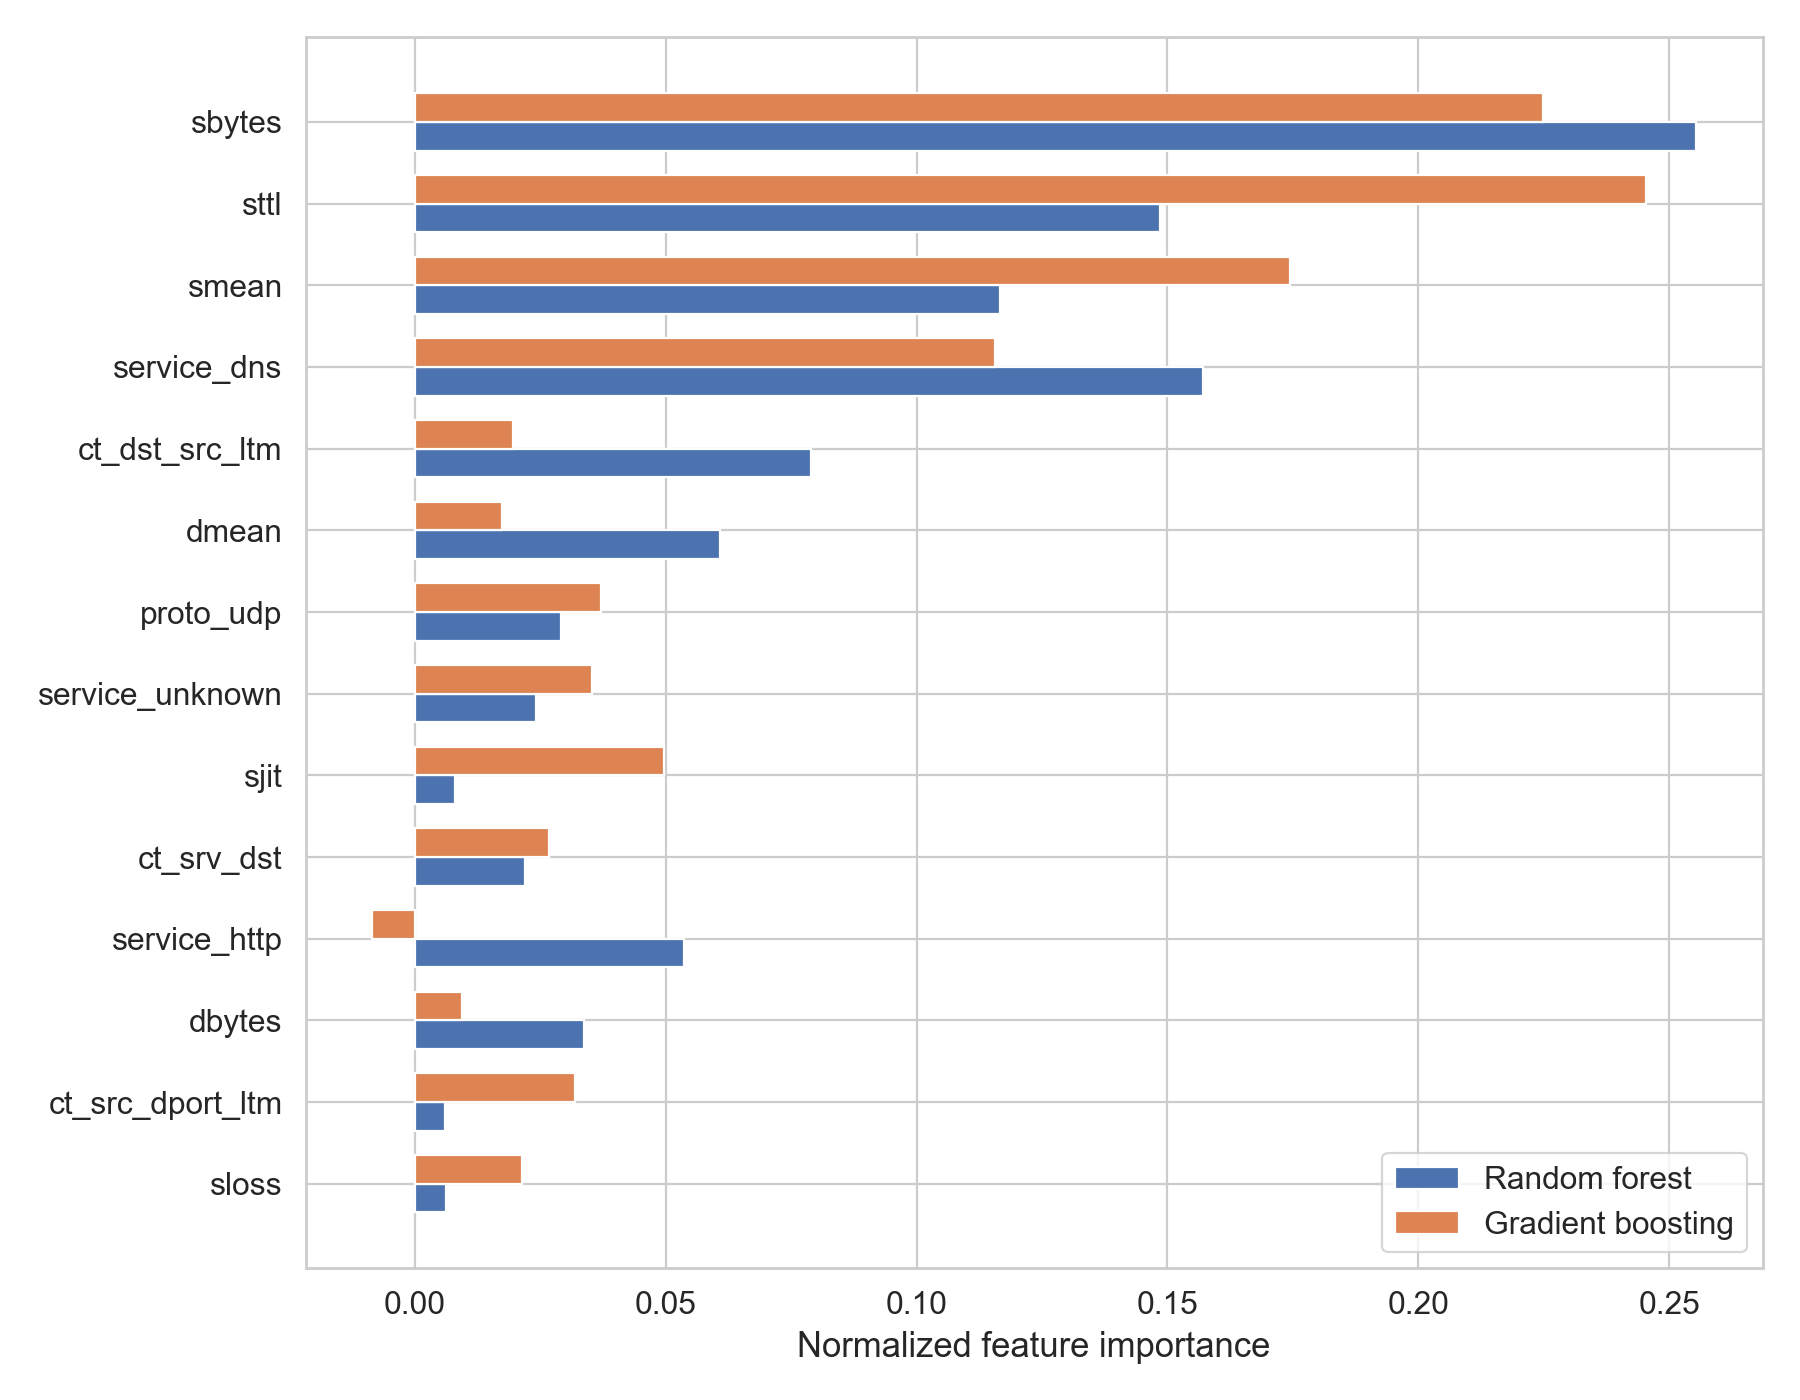
\includegraphics[width=\columnwidth]{figures/report/09_feature_importance_comparison.png}
\caption{Normalised feature importance for the most important features identified by each classifier.}
\label{fig:feature-importance}
\end{figure}

\subsection{Computational Cost}
\label{subsec:cost}
Figure~\ref{fig:computational-cost} shows the tuning time and the test set prediction time measured for the RF and GBM classifiers. The RF hyperparameter search required 6,073 seconds of tuning time, compared with 2,086 seconds for the GBM hyperparameter search. The RF classifier required 2.36 seconds to generate predictions for the 51,535 instances in the test partition, compared with 1.49 seconds for the GBM classifier. The RF classifier therefore required approximately 3 times the tuning time of the GBM classifier, and required approximately 59 percent more prediction time than the GBM classifier. This trade-off is attributed to the final tuned configuration of each classifier: the RF classifier applies 400 trees at a maximum depth of 16, while the GBM classifier applies 150 trees restricted to 15 leaf nodes each, a substantially smaller total computation per prediction.

\begin{figure}[t]
\centering
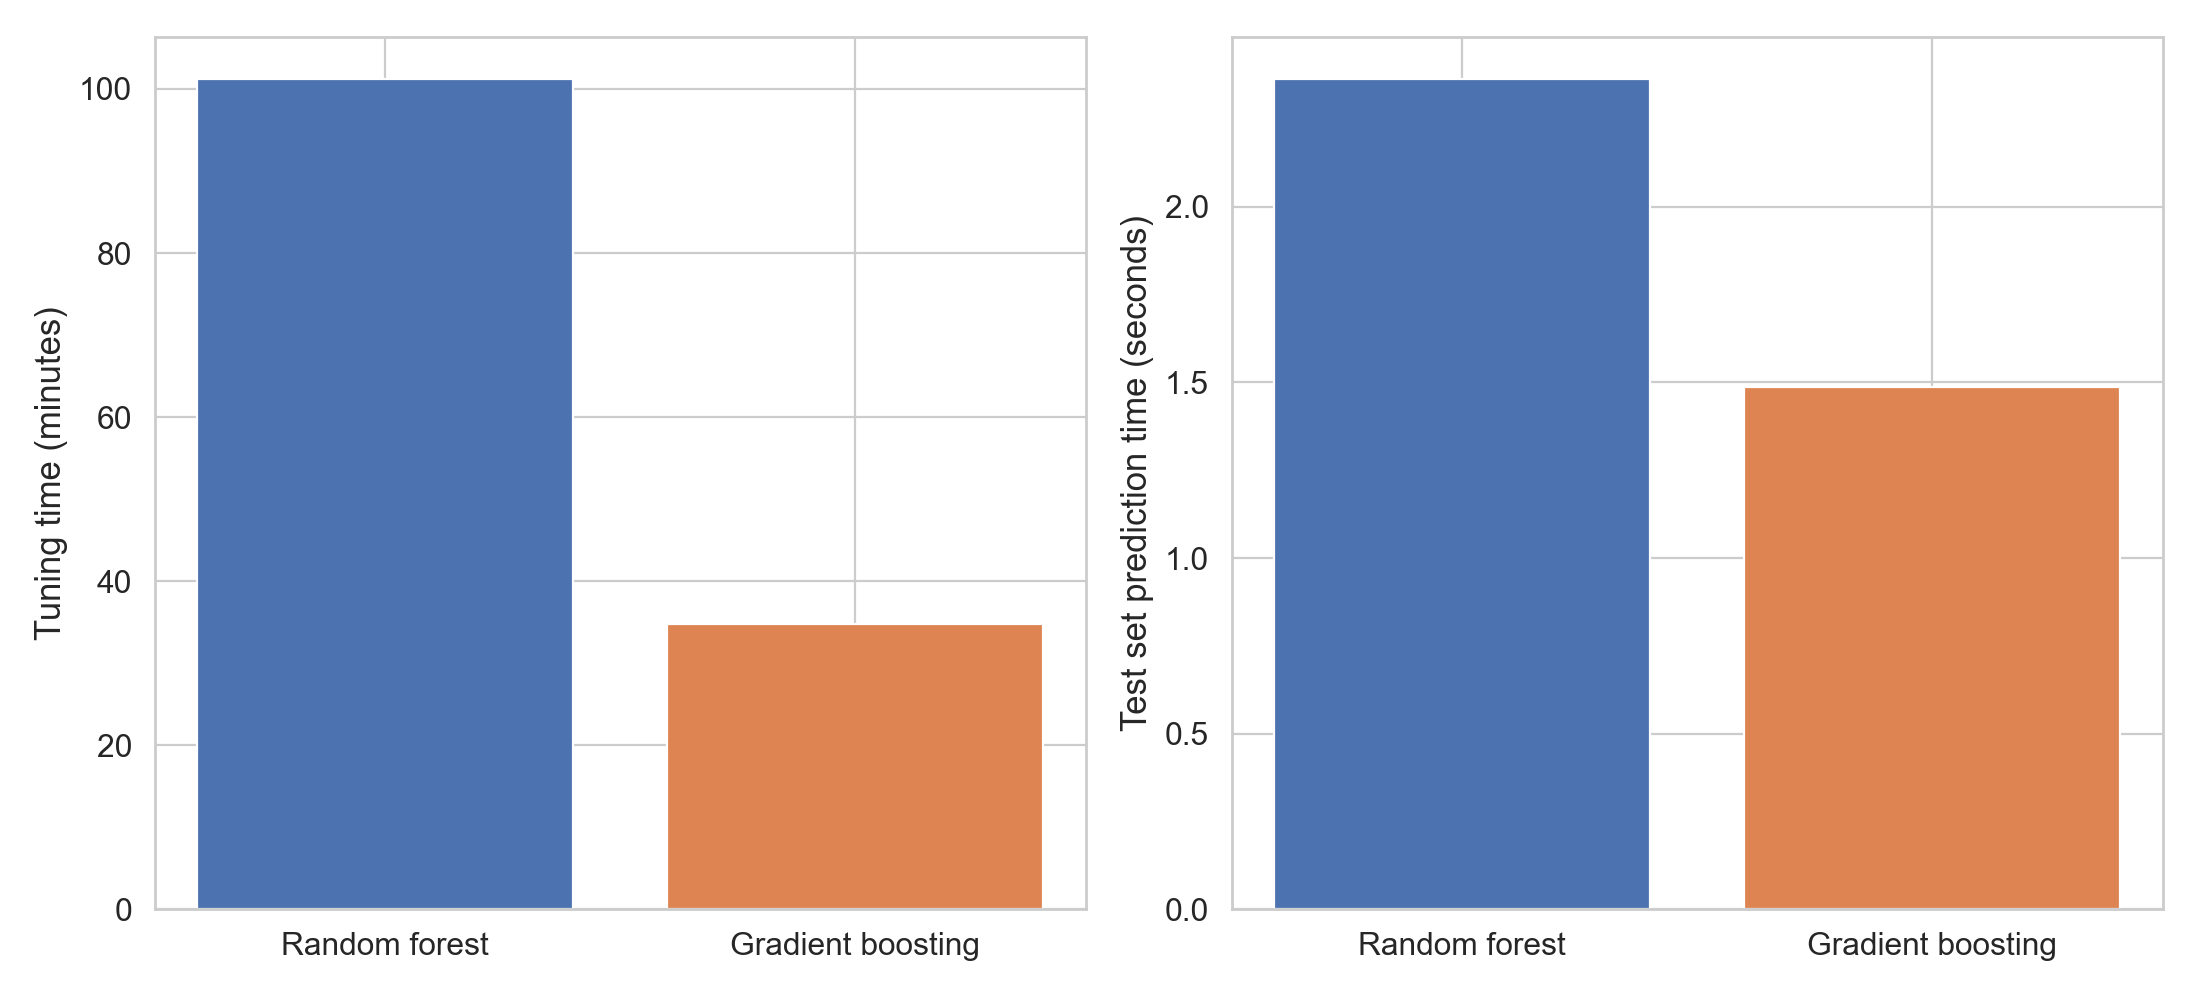
\includegraphics[width=\columnwidth]{figures/report/11_computational_cost_comparison.png}
\caption{Tuning time and test set prediction time for the RF and GBM classifiers.}
\label{fig:computational-cost}
\end{figure}

\section{Conclusions}
\label{sec:conclusion}
This report investigated the application of an RF classifier and a GBM classifier to the prediction of cyberattack categories in a severely imbalanced network traffic dataset, and compared both classifiers against a DT classifier and a kNN classifier constructed in a previous assignment on the same dataset. The RF classifier achieved the highest macro F1-score among the four classifiers compared, at 0.598, followed by the DT classifier at 0.588, the GBM classifier at 0.565, and the kNN classifier at 0.508. The small margin separating the RF classifier from a single, well-tuned DT classifier indicated that the majority of the predictive performance achieved by the RF classifier on this dataset was attributable to the base decision tree learner, with a comparatively modest additional contribution from bagging. The final tuned RF configuration applied an unrestricted number of features per split, which reduced this classifier to a bagged ensemble of decision trees rather than a random forest in the strict sense.

Both ensemble classifiers, together with the DT and kNN classifiers, performed poorly on the Backdoor and Analysis categories. This weakness was attributed to a combination of low sample counts and confusion with the Exploits and DoS categories, supported by the confusion matrix evidence presented in Section~\ref{sec:results}, and was not resolved through balanced class weighting. The consistency of this weakness across four distinct learning algorithms indicated that the weakness resulted from a property of the dataset rather than from a limitation specific to any single classifier.

A substantial gap between the CV estimate and the test estimate of generalisation performance was observed for the GBM classifier but not for the RF classifier. This gap was not fully explained by duplicate-record leakage across CV folds, because duplicate records were present in both the training partition and the test partition in a similar manner. The gap is reported as an unresolved limitation of the empirical process, and the test set result is applied as the reliable estimate of GBM performance in this report.

Future work should verify the scoring configuration applied during the GBM hyperparameter search to resolve the CV-test discrepancy identified in this report, should group duplicate flow records prior to partitioning the dataset to remove the potential for leakage identified in Section~\ref{sec:implementation}, and should investigate resampling strategies or cost-sensitive loss functions specifically targeted at the Backdoor and Analysis categories.

\appendix

\subsection{List of Acronyms}
\begin{description}
\item[CV] Cross-validation
\item[DT] Decision tree
\item[GBM] Gradient boosting machine
\item[kNN] $k$ nearest neighbours
\item[RF] Random forest
\end{description}

\subsection{List of Symbols}
\begin{description}
\item[$k$] The number of folds used during CV, or the number of neighbours considered by the kNN classifier.
\item[$K$] The number of target classes.
\item[$N$] The total number of training instances.
\item[$N_{y_i}$] The number of training instances belonging to the class of instance $i$.
\item[$w_i$] The sample weight assigned to training instance $i$.
\end{description}

\begin{thebibliography}{9}

\bibitem{beyer1999nearest}
K. Beyer, J. Goldstein, R. Ramakrishnan, and U. Shaft, ``When is nearest neighbor meaningful?'' in \emph{Proceedings of the International Conference on Database Theory}, 1999, pp. 217--235.

\bibitem{breiman1984cart}
L. Breiman, J. H. Friedman, R. A. Olshen, and C. J. Stone, \emph{Classification and Regression Trees}. Boca Raton, USA: Chapman and Hall, 1984.

\bibitem{breiman1996bagging}
L. Breiman, ``Bagging predictors,'' \emph{Machine Learning}, vol. 24, no. 2, pp. 123--140, 1996.

\bibitem{breiman2001randomforest}
L. Breiman, ``Random forests,'' \emph{Machine Learning}, vol. 45, no. 1, pp. 5--32, 2001.

\bibitem{cover1967knn}
T. Cover and P. Hart, ``Nearest neighbor pattern classification,'' \emph{IEEE Transactions on Information Theory}, vol. 13, no. 1, pp. 21--27, 1967.

\bibitem{friedman2001gradientboosting}
J. H. Friedman, ``Greedy function approximation: A gradient boosting machine,'' \emph{Annals of Statistics}, vol. 29, no. 5, pp. 1189--1232, 2001.

\bibitem{geman1992biasvariance}
S. Geman, E. Bienenstock, and R. Doursat, ``Neural networks and the bias/variance dilemma,'' \emph{Neural Computation}, vol. 4, no. 1, pp. 1--58, 1992.

\bibitem{ke2017lightgbm}
G. Ke, Q. Meng, T. Finley, T. Wang, W. Chen, W. Ma, Q. Ye, and T.-Y. Liu, ``LightGBM: A highly efficient gradient boosting decision tree,'' in \emph{Proceedings of the Conference on Neural Information Processing Systems}, 2017, pp. 3146--3154.

\bibitem{moustafa2015unsw}
N. Moustafa and J. Slay, ``UNSW-NB15: A comprehensive data set for network intrusion detection systems,'' in \emph{Proceedings of the Military Communications and Information Systems Conference}, 2015, pp. 1--6.

\bibitem{strobl2007bias}
C. Strobl, A.-L. Boulesteix, A. Zeileis, and T. Hothorn, ``Bias in random forest variable importance measures: Illustrations, sources and a solution,'' \emph{BMC Bioinformatics}, vol. 8, article 25, 2007.

\end{thebibliography}

\end{document}